% interactnlmsample.tex
% v1.05 - August 2017
% Alan Revisions Dec 19, 2017

% \PassOptionsToPackage{dvipdfmx}{graphicx}
% \PassOptionsToPackage{dvipdfmx}{rotating}
\documentclass[]{interact}

% interact.cls includes:
% \RequirePackage{amsmath,amssymb,amsfonts,amsbsy,amsthm,booktabs,epsfig,graphicx,rotating}

%-------------------------------------- interact required packages -----------------------------------------------
% \usepackage{epstopdf} % To incorporate .eps illustrations using PDFLaTeX, etc.
%%%% Yamada removed this b/c he has no eps figures, only jpg and png

% \usepackage[caption=false]{subfig}% Support for small, `sub' figures and tables
%%%% in order to \usepackage{subfigure}
%\usepackage[nolists,tablesfirst]{endfloat}% To `separate' figures and tables from text if required
%\usepackage[doublespacing]{setspace}% To produce a `double spaced' document if required
%\setlength\parindent{24pt}% To increase paragraph indentation when line spacing is doubled

\usepackage[numbers,sort&compress]{natbib}% Citation support using natbib.sty
\bibpunct[, ]{[}{]}{,}{n}{,}{,}% Citation support using natbib.sty
\renewcommand\bibfont{\fontsize{10}{12}\selectfont}% Bibliography support using natbib.sty
\makeatletter% @ becomes a letter
\def\NAT@def@citea{\def\@citea{\NAT@separator}}% Suppress spaces between citations using natbib.sty
\makeatother% @ becomes a symbol again

\theoremstyle{plain}% Theorem-like structures provided by amsthm.sty
\newtheorem{theorem}{Theorem}[section]
\newtheorem{lemma}[theorem]{Lemma}
\newtheorem{corollary}[theorem]{Corollary}
\newtheorem{proposition}[theorem]{Proposition}

\theoremstyle{definition}
\newtheorem{definition}[theorem]{Definition}
\newtheorem{example}[theorem]{Example}

\theoremstyle{remark}
\newtheorem{remark}{Remark}
\newtheorem{notation}{Notation}

%------------------------------------ Author Requested Packages -----------------------------------------------   
\RequirePackage{fix-cm} % removes some restrictions on size of CM and EC fonts
% \smartqed  % flush right qed marks, e.g. at end of proof
%
% \usepackage{bmpsize}
% \usepackage[dvipdfmx]{graphicx} % 

% \usepackage{graphicx} % Required by interact.cls

% \usepackage[round]{natbib}
%
% \usepackage{mathptmx}      % use Times fonts if available on your TeX system
%
\usepackage{algorithm,algorithmicx,algpseudocode}
 \usepackage{subfigure} 
% \usepackage{amsmath,mathtools,amssymb,eucal,bbm,bm}
\usepackage{mathtools,eucal,bm}
% bbm removed b/c didn't work w/journal; bbm only required to get nice looking Real symbol
% amssymb is good enough Real symbol
\usepackage{bigstrut} % make table vertical spacing bigger
\usepackage{afterpage}
% \usepackage[titletoc,title]{appendix}
% etc.
%
% please place your own definitions here and don't use \def but
% \newcommand{}{}
%
% Insert the name of "your journal" with
% \journalname{Journal of Statistical Computation and Simulation}
%

%%% \AtBeginDocument{%  This fixes the margin and text widths; but delete before submission
%%%     \paperwidth=\dimexpr
%%%       1in + \oddsidemargin
%%%     + \textwidth
%%%     % + \marginparsep + \marginparwidth
%%%     + 1in + \oddsidemargin
%%%   \relax
%%%   \paperheight=\dimexpr
%%%     1in + \topmargin
%%%     + \headheight + \headsep
%%%     + \textheight
%%%     % + \footskip
%%%     + 1in + \topmargin
%%%   \relax
%%%   \usepackage[pass]{geometry}\relax
%%% }

%------------------------------------------------------------------------------------------
\begin{document}

\articletype{ARTICLE TEMPLATE} % Specify the article type or omit as appropriate

%------------------------------------------------------------------------------------------             Title

\title{An algorithm for nonparametric estimation of a  multivariate
               mixing distribution}

\newif\ifanonymous
\anonymoustrue

\ifanonymous
\else
% \author{
% \name{A.~N. Author\textsuperscript{a}\thanks{CONTACT A.~N. Author. Email: latex.helpdesk@tandf.co.uk} and John Smith\textsuperscript{b}}
% \affil{\textsuperscript{a}Taylor \& Francis, 4 Park Square, Milton Park, Abingdon, UK; \textsuperscript{b}Institut f\"{u}r Informatik, Albert-Ludwigs-Universit\"{a}t, Freiburg, Germany}
% }

\author{
\name{
Walter M. Yamada\textsuperscript{a}$^\ast$\thanks{$^\ast$CONTACT W.~M. Yamada. Email: wyamada@chla.usc.edu}
\and Michael N. Neely\textsuperscript{a}\textsuperscript{b} 
\and David S. Bayard\textsuperscript{c} 
\and James V. Burke\textsuperscript{d} 
\and Mike van Guilder\textsuperscript{a} 
\and Roger W. Jelliffe\textsuperscript{a} 
\and Alona Kryshchenko\textsuperscript{a}\textsuperscript{e}$\dagger$\thanks{$\dagger$CONTACT A. Kryshchenko. Department of Mathematics, California State University Channel Islands,  1 University Dr, Camarillo, CA 93012, USA}
\and Robert Leary\textsuperscript{f} 
\and Alan Schumitzky\textsuperscript{e}$\ddagger$\thanks{$\ddagger$CONTACT A. Schumitzky. Tel.:+1 818-249-9444. Fax:+1 213-740-2424. Email: schum@usc.edu}
}
%
\affil{
 \textsuperscript{a}Laboratory of Applied Pharmacokinetics and Bioinformatics, Children's Hospital of Los Angeles,  Los Angeles, CA 90027, USA;
\and
\textsuperscript{b}Pediatric Infectious Diseases, Children's Hospital of Los Angeles, Keck School of Medicine, University of Southern California, Los Angeles, CA 90027, USA; % \\ \email{mneely@chla.usc.edu}
\and
\textsuperscript{c}Jet Propulsion Laboratory, California Institute of Technology, Pasadena CA, 91109, USA; % \\ \email{dbay007@earthlink.net,}
\and
\textsuperscript{d}Department of Mathematics, University of Washington, Seattle, WA  98195, USA; % \\ \email{jvburke@uw.edu}
% \and M. van Guilder \at \email{uphill@cox.net} \and R.W. Jelliffe \at \email{jelliffe@usc.edu}
\and 
\textsuperscript{e}Department of Mathematics, University of Southern California, Los Angeles, CA 90089, USA;
%Department of Mathematics, California State University Channel Islands,  University Dr, Camarillo, CA 93012, USA; % \\\email{achubatyuk@gmail.com}
\and
\textsuperscript{f}Certara, Raleigh, NC 27606, USA; %  \\\email{Bob.Leary@certara.com}
%% \and
%% \textsuperscript{g}Department of Mathematics, University of Southern California, Los Angeles, CA 90089, USA %\\Tel.:+1 818-249-9444; Fax:+1 213-740-2424 \\\email{schum@usc.edu}
}} % END of \author INFORMATION
\fi

\maketitle

%------------------------------------------------------------------------------------------             Abstract

\begin{abstract}
In this paper we describe a nonparametric maximum likelihood (NPML) algorithm for estimating multivariate mixing distributions. Given $N$ independent observations, convexity theory shows that the NPML estimator is discrete with at most $N$ support points. The original infinite NPML problem then becomes the finite dimensional problem of finding the location and probability of the support points. The probability of the support points is found by a Primal-Dual Interior-Point method; the location of the support points is found by an Adaptive Grid method. Our method is able to handle high-dimensional and complex multivariate mixture models.  An important application is discussed for the problem of population pharmacokinetics and a non-trivial example is treated. In addition to population pharmacokinetics, this research also applies to empirical Bayes estimation and many other areas of applied mathematics.
\end{abstract}

\begin{abbreviations}
IPM; NPAG; NPML
\end{abbreviations}

\begin{keywords}
% Multivariate mixing distributions;
High dimensional statistics;
Nonparametric maximum likelihood;
Primal-dual interior-point method;
Adaptive grid
% \and Population pharmacokinetics
\end{keywords}

{\bf WORD COUNT = 5084}

%------------------------------------------------------------------------------------------             Body of Paper 

\section{Introduction} \label{Section:Introduction}
    % Introduction_v13

%%%
The mixing distribution problem we consider can be stated as follows.
%
Let $\bm{Y}_1, ... , \bm{Y}_N$ be a sequence of independent but not necessarily identically distributed random vectors % .
%
% Each $\bm{Y}_i$ is a matrix of
constructed from one or more observations from each of $N$ subjects in the population.
%
Let $\bm{\theta}_1,...,\bm{\theta}_N$ be a sequence of independent and identically distributed 
% $Q$-dimensional 
random vectors belonging to a  compact subset $\Theta$ of Euclidean space with common but {\em unknown} distribution $F$.
%
The $\{\bm{\theta}_i\}$ are not observed.
%
It is assumed that the conditional densities $p(\bm{Y}_i \vert \bm{\theta}_i)$ are known, for $i = 1,...,N$.
%
The mixing distribution of $\bm{Y}_i$ with respect to $F$ is given by $p(\bm{Y}_i \vert F ) = \int p(\bm{Y}_i \vert \bm{\theta}_i ) dF(\bm{\theta}_i)$.
%
Because of independence of the $\{\bm{Y}_i\}$, the mixing distribution of the $\{\bm{Y}_i\}$ with respect to $F$ is given by
%
\begin{equation}
	L(F) = p(\bm{Y}_1,...,\bm{Y}_N \vert F) = \prod_{i=1}^N \int p \left(\bm{ Y}_i \vert \bm{\theta}_i \right) dF\left( \bm{\theta}_i \right)
\end{equation}
%
{\em The mixing distribution problem is to maximize the likelihood function  $L(F)$ with respect to all probability distributions $F$ on $\Theta$.}

%%%
Remark.
%
The distribution $F^{ML}$ that maximizes $L(F)$ is a {\em consistent} estimator of the true mixing distribution. This was proved originally by 
Kiefer and Wolfowitz in 1956
 \cite {Kiefer1956} . %Kiefer and Wolfowitz (1956). %in 1956 \cite {Kiefer1956}. 
%
The consistency of $F^{ML}$ is especially important for our application to population pharmacokinetics where  $F^{ML}$ is used as a prior distribution for Bayesian dosage regimen design.


%%%
The algorithm described in this paper differs from most other published methods in a number of ways. Our algorithm allows for high dimensional $\Theta$.  
%
Most published methods require the dimension of $\Theta$ to be small and many require the dimension of $\Theta$ to be 1, see Section \ref{Section:Other_algorithms}. 
%
We have treated examples where the dimension of $\Theta$ is as high as 29, 
%although in this case the run time took months, 
see Section \ref{Section:Examples}.
%

Also most published algorithms require the $\{\bm{Y}_i\}$ to be identically distributed and assume that the conditional densities $\{p(\bm{Y}_i \vert \bm{\theta}_i)\}$ 
are rather simple, such as $p(\bm{Y}_i \vert \bm{\theta}_i)$ is a multivariate normal density with mean vector and covariance matrix $\bm{\Sigma}$.
%
%= $N(\theta,\sigma^2)$, in the univariate case or $p(Y_i \vert \theta_i)$ = $N(\theta,\Sigma)$ in the multivariate case. (Here and in what follows, $N(\mu,\Sigma)$ will mean a normal distribution with mean vector $\mu$
%and covarince matrix $\Sigma$.) 
%
Even if $\bm{\Sigma}$ is unknown and has to be estimated, the structure of this model is straightforward. However, the estimation of $\bm{\Sigma}$ has to be done carefully to avoid singularities, see Wang and Wang \cite{Wang2015}.
As will be described in Section \ref{Section:Examples}, we allow  $p(\bm{Y}_i \vert \bm{\theta}_i)$ to be calculated from a  system of nonlinear ordinary differential-algebraic  equations.

%%%
We now describe the details of our algorithm. It was proved by
\citet {Lindsay1983} and \citet {Mallet1986} , 
under simple hypotheses
on the conditional densities $\{p(\bm{Y}_i \vert \bm{\theta}_i)\}$, that  the global maximizer $F^{ML}$ of $L(F)$ could be represented by a discrete distribution with at most $N$ support points.

%Eq. (\ref{Eqn:Likelihood002}) is the starting point of many NPML algorithms.

%
This result leads immediately to a finite dimensional optimization problem for $F^{ML}$, namely to maximize the likelihood function
\begin{equation}
%\begin
	L( \bm{\lambda}, \bm{\phi}) =\prod_{i=1}^N \sum_{k=1}^K  \lambda_k p\left( \bm{Y}_i \vert  \bm{\phi}_k \right)
%\end
\label{Eqn:Likelihood001}
\end{equation}
with respect to the support points $\bm{\phi} = ( \bm{\phi}_1, ... ,  \bm{\phi}_K)$ 
and weights $ \bm{\lambda} = ( \lambda_1, ... ,\lambda_K)$  such that 
$  \bm{\phi}_k \in \Theta, \lambda_k \geq 0$
for $k=1, ... , K$, $K \leq N$ and \; $\sum_{k=1}^K   \lambda_k = 1$. 

% In the above equation and in what follows, for any symbol $\alpha$, we will use the notation $\bar \alpha$ to indicate  $\bar \alpha=(\alpha_1, ... ,\alpha_n)$ for some $n$

In our algorithm $l(\bm{\lambda},\bm{\phi})=\log L(\bm{\lambda},\bm{\phi})$ is maximized, so that
%In our algorithm $l(\bf \lambda,\bar\phi)=\log L(\mathbf{ \lambda},\bar \phi)$ is maximized, so that
\begin{equation}
	l(\bm{\lambda},\bm{\phi}) =\sum_{i=1}^N \log \sum_{k=1}^K  \lambda_k p\left( \bm{Y}_i \vert  \bm{\phi}_k \right)
\label{Eqn:Likelihood001b}
\end{equation}
and the maximization problem becomes
%\[
%	 \quad \mbox{maximize} \; l \left( \bar \lambda, \bar \phi \right) \; \mbox{s.t.} \;
% 0 \le \bar \lambda, \; e^T\bar \lambda = 1,
%\]
\begin{equation}
\mbox{maximize} \;  l(\bm{\lambda},\bm{\phi})
\label{Eqn:Likelihood002}
\end{equation}
such that $\bm{\phi} \in \Theta^K$, $\bm{\lambda} = ( \lambda_1, ... , \lambda_K) \in \mathbb{R}_+^K$, $K \leq N$  and \; $\sum_{k=1}^K   \lambda_k = 1$.



Although the maximization problem in Eq. (\ref{Eqn:Likelihood002}) is finite dimensional, it is still high dimensional.
%
The dimension of the maximization problem in Eq. (\ref{Eqn:Likelihood002}) is $N (\dim{\Theta}) + (N - 1)$.

The optimization problem in Eq. (\ref{Eqn:Likelihood002}) is naturally divided into two problems:
%\begin{enumerate}[leftmargin=0cm]
%\item 

%[Problem 1)] 
Problem 1. Given a set of support points $\{ \bm{\phi}_k\}$, find the optimal weights $\{ \lambda_k\}$.
%\item [Problem 2)] 

Problem 2. Find the locations of the optimal support points 
%\end{enumerate}
%

Problems  1 and 2 are solved cyclically until convergence, i.e. no significant improvement in $l( \bm{\lambda},\bm{\phi})$.


%%%
Problem 1 is a convex programming problem.
%
In our algorithm, we solve this problem by the Primal-Dual Interior-Point (PDIP) method.
%
This type of method is standard in convex optimization theory, see Boyd and Vandenberghe \cite{Boyd2004}.
%
However, the exact implementation for a specific problem varies from problem to problem.
%
The exact details of our implementation is described in the Appendix.
%
See also \citet{Bell2012b:Online}, \citet{Baek2006}  and \citet{LAPK-2014-01}.
%See also \citet{Bell2012b:Online,Baek2006}, {LAPK-2014-01}.
% See also Bell (2012), Baek (2006) and  Yamada et al. (2014). 
%
Our PDIP implementation is very fast and can easily handle thousands of variables.

%%%
% The main contribution of this paper is the solution to Problem 2.  
Finding the  location of the optimal support points in Problem 2 is a more difficult  problem. This location problem is a non-convex global optimization problem with many local extrema and whose dimension is potentialy $N \times \dim{\Theta}$. % $N \times  Q$.
%
The details of our algorithm, called the Adaptive Grid (AG) method, will be described in Section \ref{Section:Adaptive_Grid_Method} and in Algorithm 1.
%
Roughly speaking, an initial large grid of possible support points is defined in $\Theta$.
%
Problem 1 is  solved on this large grid. 
%
After PDIP, most of the original grid points are removed due to near-zero weights leaving a smaller high-probability grid.
%
Problem 1 is then solved on this smaller grid.
%
Then the adaptive step takes place.
%
For each remaining  grid point, up to $2 \times {\dim{\Theta}}$ new (daughter) support points are added.
%
A daughter point outside the search space $\Theta$ or too close to a parent point is discarded.
%
The new grid contains the current high-probability points plus the added daughter points.
%
The algorithm is then ready for Problem 1, again.
%
By construction, each iteration increases the value of $l(\bm{\lambda}, \bm{\phi})$. 
%
This process continues until the function $l(\bm{\lambda},\bm{\phi})$ does not significantly change.

%Remark. The result of Lindsay and Mallet that $F^{ML}$ was represented by a discrete distribution with at most $N$ support points marked the beginning of most of the recent developments in NPML algorithms.
%It is surprising to note that  a similar result holds even without the optimization step. It can be shown that {\em every} feasible distribution for the optimization problem of Eq. 1 can be represented by a discrete distribution with at most $N+1$ support points.
% can be represented by a discrete distribution $F$ with at most $N+1$ support points. 
%
%This later result is a consequence of the Krein-Milman theorem for compact convex  sets
%and Carath$\acute{e}$odory's theorem, see \cite{Lindsay1983,  Baek2006, Phelps1966}. The optimization step then just reduces the number of support points by $1$.
%
% integral of the form $\int p \left( Y_i \vert \theta
%Simon B. Convexity: An Analytic Viewpoint. Cambridge University Press, 2011.


%%% End Introduction_v12
\section{Other algorithms} \label{Section:Other_algorithms}
    
%\section{Other algorithms}

\subsection{Comparable Methods}

Because of space limitations, in this section we only discuss NPML methods that optimize Eq. \ref{Eqn:Likelihood002}; methods that treat multivariate distributions; and methods which allow general conditional probabilities 
$\{P(\bm{Y}_i, \bm{\theta}_i)\}$.
%
As explained in this paper, any such NPML algorithm has to address two problems: {\em locations} of support points and {\em weights} of support points.
%
NPAG does {\em locations} by an Adaptive Grid method and {\em weights} by the Primal-Dual Interior-Point (PDIP) method.
%

The original methods of Lindsay \cite{Lindsay1983}  and Mallett  
\cite{Mallet1986} 
were based on algorithms of optimal design in the style of \citet{Fedorov1972}. % Fedorov (1972). %. 
%In 1991, Schumitzky proposed an algorithm  which did both {\em locations} and {\em weights} by the EM algorithm, see Schumitzky(1991). It was very stable but also very slow. 
In Schumitzky
\cite{Schumitzky1991},
an algorithm  was proposed which did both {\em locations} and {\em weights} by the EM algorithm.  It was very stable but also very slow. 

In  \citet{Lesperance1992},  a new method was introduced  %\cite{Lesperance1992}.  
which did  {\em weights}  by the dual method described in Section 5 of  \citet{Lindsay1983} 
and {\em locations} by what they called the Intra-Simplex Direction Method (ISDM). Even though, the Lesperance and Kalbfleisch paper was restricted to univariate distributions, the ISDM method has been generalized to the multivariate case. To briefly describe ISDM, let  $D(\bm{\theta},F)$ be the directional derivative of   $\log L(F)$ in the direction of the Dirac distribution $\delta_{\bm{\theta}}$ supported at $\bm{\theta}  \in \Theta$.  (This function is defined in Section 4 below.)  ISDM is an iterative algorithm. At stage $k$, let $F^k$ be the current estimate $F^{ML}$. Then find all the local maxima  of $D(\bm{\theta}, F^k)$.  These local maxima are added to the current set of support points and a new $F^{k+1}$
is calculated. If there are no new local maxima, then the algorithm is done.

%%%
%Most of the algorithms so far developed in the literature use some combination of the above methods.
%


In  \citet*{Pilla2006}, another new method was developed where
%Pilla, Bartolucci and Lindsay
the {\em locations} were found by an initial fine grid. But the   {\em weights} were found by a dual version of the PDIP method.
% Finding the weights by the PDIP method is an $N$ dimensional problem, where $N$ is the number of subjects. Using the method in \cite{Pilla2006}, the finding the weights is  a $Q$-dimensional problem, where $Q$ is the dimension of $\Theta$.  $N$ is always much bigger than $Q$.
%(In the pharmacokinetc problem in Section 5, $N=300$ while $Q=5$

In  \citet* {Savic1},
%Savic, Kjellsson and  Karlsson(2009), 
a nonparametric method was added to the popular NONMEM program. NONMEM-NP   is a hybrid parametric-nonparametric approach %\cite{Savic1}.
The {\em locations} of support points were found by a parametric maximum likelihood algorithm. Then the {\em weights} were found by maximizing Eq. (4) relative to the newly found support points. 
NONMEM-NP can handle high dimensional and complex multivariate distributions. An extension to NONMEM-NP was developed in %\cite{Savic2009c}
\citet{Savic2}
where additional support points are added to the original set. A comparison between NONMEM-NP and NPAG is discussed in \citet*{Leary2017}.

%In 2015, 

In % Wang and Wang (2015),
\citet{Wang2015} ,
a new algorithm was developed for multivariate distributions. The {\em locations} were found by a combination of EM and a variant of ISDM. The {\em weights} were found by a family  of Quadratic Programs.  In \cite{Wang2015}, examples are done for 8 and 13 dimensional mutivariate mixing distributions. 
%Clearly the problem of finding local maxima of $D(\bm{\theta},F)$ is much easier in 1 dimension than in 8 or 13 dimensions.

Note: The Quadratic Programming algorithm (QP) of  \citet{Wang2015} has a very attractive feature. For a prescribed set of support points, QP finds the zero probabilities exactly. Thus QP avoids the Grid Condensation step where support points from PDIP with sufficiently low probabilities are deleted. However, QP and PDIP are based on different numerical methods and a comparison of the efficiency of both algorithms has not been determined.

The algorithms which have shown by published examples to handle the highest dimensional multivariate problems are NONMEM NP, \citet{Wang2015},  and NPAG.




\subsection{Benders Decomposition}
For any set of grid points $\bm{\phi} = (\bm{\phi}_1, ...,\bm{\phi}_m)$ in $\Theta^m$, 
let $\bm{\lambda} = \bm{\hat{\lambda}}(\bm{\phi})$
 be the corresponding set of optimal weights given by the PDIP  method.
Then the function $F(\bm{\phi}) =l( \bm{\hat{\lambda}}(\bm{\phi}),\bm{\phi})$ depends only on $\bm{\phi}$  and can be maximized directly.
For optimization methods,  this technique  is called Benders Decomposition. The NPAG algorithm maximizes $F(\bm{\phi})$ by an adaptive search method. In a method proposed by James Burke, $F(\bm{\phi})$ is maximized  by a Newton type method. Since the function  $F(\bm{\phi}$) is not necessarily differentiable, a relaxed Newton method must be used similar to what is described in the Appendix for the Primal-Dual Algorithm. For details of Benders Decomposition as applied to our problem,  see  \citet{Baek2006, Bell2012b:Online}  and \citet{Squire2015}.
%\cite{Bell2012b:Online, Baek2006}.




\section{Adaptive Grid Method} \label{Section:Adaptive_Grid_Method}
    %%%%%%%%%%%%%%%%%%%%%%%%%%%%%%%%%%%%%%%%%%%%%%%%%%%%%%%%%%%%%%%%
%
%                                                                  Section NPAG
%
%%%%%%%%%%%%%%%%%%%%%%%%%%%%%%%%%%%%%%%%%%%%%%%%%%%%%%%%%%%%%%%%

\subsection{NPAG Implementation (NPAG - Algorithm 1)}
\label{NPAG}

NPAG is a Fortran program consisting of a number of subroutines as described below.
%
The main program performs the Adaptive Grid (AG) method (consisting of expansion and compression algorithms) and calls the Primal-Dual Interior-Point (PDIP) subprogram.
% .  The AG program calls the Primal-Dual Interior-Point (PDIP)  subprogram.
The PDIP algorithm solves the maximization problem  of Eq. (\ref{Eqn:Likelihood002}) for a fixed grid and is  described precisely in the Appendix. 

For the purpose of this discussion, we can think of PDIP as a function  $\bm{\hat{\lambda}}$ from $\Theta^m$ into the set $S^m$ = $\{\bm{\lambda}  \in \mathbb{R}_{+}^{m}:  \sum_{k=1}^m  \lambda_k = 1 \}$
%$(m-1)$-dimensional simplex $S^{m}$, 
defined as follows:
%
If  $\bm{\phi} = (\bm{\phi}_1, ... , \bm{\phi}_m)$ then $\bm{\hat{\lambda}}(\bm{\phi})= (\hat{\lambda}_1, ... ,\hat\lambda_m)$
maximizes Eq. (\ref{Eqn:Likelihood002})  relative to the fixed set of grid points $(\bm{\phi}_1, ... , \bm{\phi}_m)$. 
In this case we write  $G$ = $(\bm{\phi},\bm{\hat{\lambda}}(\bm{\phi}))$  and  $l(G)$ = $l(\bm{\phi}, \bm{\hat{\lambda}}(\bm{\phi}))$.

In NPAG there are two types of grids: expanded and condensed. The expanded grids are the initial grid and the grids after Grid Expansion (Algorithm 2).
The condensed grids are generated by Grid Condensation (Algorithm 3). % Except for the last cycle, the likelihood calculation is done on the expanded grids.
Each cycle of NPAG begins with an expanded grid. The likelihood calculation is done on the condensed grids.

%%%
Now for the Adaptive Grid method.
%
Assume that $ \Theta$  is  a bounded $Q$-dimensional hyper-rectangle.
%
Initially we let  $\bm{\phi}^{0}_{expanded} = (\bm{\phi}^{0}_1, ... , \bm{\phi}^{0}_M)$ be the set of $M$ Faure grid points in $\Theta$, see
\cite{FaureSequence, InitFaureSequence, DoFaureSequence}.
%
Alternatively, we could initially let $\bm{\phi}^0_{expanded}$ be generated by a uniform distribution on  $\Theta$ or by a prior run of the program.

Remark. The Faure grid points for a hyper-rectangle $\Theta$ are a low-discrepancy set which in some sense optimally and uniformly covers $\Theta$.  In our implementation of NPAG, the Faure point sets come in discrete sizes which nest with each other.  (Allowable number of  points equals 2129,  5003, 10007,  20011,  40009, 80021, and multiples of 80021.) This nesting property  is useful for checking the optimality of  $F^{ML}$, see Section 4. We have found that replacing the initial Faure set by a set generated by a uniform distribution on  $\Theta$
increases the time to convergence but results in the same optimal distribution. 

%In Figure XXX, a side-by-side examplesof a Faure set on 
%$[0,1] \times [0,1]$ and a set generated by a uniform distribution
%are displayed.

Now set $G^0_{expanded}$ = $(\bm{\phi}^0,\bm{\hat\lambda}(\bm{\phi}^0))$.
%
Our approach is to generate a sequence of solutions $G^n$ to Eq. (\ref{Eqn:Likelihood002}) of increasingly greater likelihood,
where unless otherwise specified, $ G^n $ refers to the condensed grid at the $n^{th}$ cycle of the algorithm.
%, and stopping when evaluation of $G^{n}$ is negligibly different than evaluation of $G^{n-1}$.
%
%At that point, $G^n$ is considered a {\em potential} optimal solution to Eq. (\ref{Eqn:Likelihood002}), and $l(G^n)$ is saved as $F_0$.
%
%$\bm{\phi}^n$ is then used as a seed to generate a new $\bm{\phi}^0$, which is used to begin a new sequence.
%
If  $ G^n $ has log likelihood negligibly different than  $ G^{n-1} $, then $ G^n$  is considered the optimal solution to Eq. (\ref{Eqn:Likelihood002}) and is relabeled $F^{ML}$.
%
If not, then the process continues using the $\bm{\phi}^n$ as the new seed.
%
This loop is repeated until $F^{ML}$ is found.


The stopping conditions for NPAG are defined precisely in Algorithm 1.
If the stopping conditions are not met prior to a set maximum number of iterations, the program will exit after writing the last calculated  $G^n$ into a file.
%

%%%%%%%%%%%%%%%%%%%%%%%%%%%%

\subsection{Grid Expansion (EXPAND - Algorithm 2)}
\label{SS:GridExpansion} 

The crux of the Adaptive Grid method is how to go from $G^0$ to $G^1$ or more generally, from $G^n$ to $G^{n+1}$.
%%%
%
The details of doing this are now explained roughly below and precisely in Algorithm \ref{OuterLoopOfNPAG}.
%see also Algorithms \ref{GridExpansionAlg} and \ref{Algorithm:PDIP}.

Let $Q$ be the dimension of $\Theta$.  Suppose at stage $n$ we have a grid of high-probability support points 
$\bm{\phi}^n$. We then add $2Q$ daughter points for each support point   $\bm{\phi}_k \in \bm{\phi}^n$. 
%%
The daughter points are the vertices of a small hyper-rectangle centered at each $\bm{\phi}_k$ with size proportional to the original size of the hyper-rectangle defining $\Theta$. The size of this small hyper rectangle decreases as the accuracy of the estimates increases. (See Algorithm 2.) 

Let $\bm{\phi}^{n+1}_{expanded}$ = $\bm{\phi}^n \cup \mbox{Daughter-Points}$.
Then the PDIP subprogram is applied to $\bm{\phi}^{n+1}_{expanded}$ resulting in the
new solution set $G^{n+1}_{expanded}$ =  $(\bm{\phi}^{n+1}_{expanded},\bm{\hat\lambda} (\bm  {\phi}^{n+1}_{expanded}  )  )$; 
see Algorithm \ref{OuterLoopOfNPAG}. The solution set $G^{n+1}_{expanded}$ is now ready for grid condensation.

%%% %%%
\subsection{Grid Condensation (CONDENSE - Algorithm 3)}
The above solution set $G^{n+1}_{expanded}$   may have many support points with very low probability.
We remove all support points which have corresponding probability less than 
%( $\bm{\lambda} > (\max\bm{\lambda})\Delta_\lambda $ )}$
$(\max\bm{\lambda}) \Delta_{\bm{\lambda}}$, where $\bm{\lambda}$ is the vector of current probabilities and  the 
default for  $\Delta_{\bm{\lambda}}$  is $10^{-3}$.  (Note that at this point the remaining probabilities are not normalized.)
%
The probabilities of the remaining support points are normalized by a second call to the PDIP subprogram.
%
This second call to PDIP is very fast.
%
The likelihood associated with these remaining support points and normalized probabilities is then used to update the program control parameters and check for convergence (Algorithm \ref{OuterLoopOfNPAG} and Section \ref{SS:Convergence}).
If convergence is attained, then the output of this second call to PDIP provides the support points and probabilities of the final solution.
If convergence is not attained, then the remaining support points are sent to the Grid Expansion subprogram (Algorithm 2), initializing the next cycle.
%

At the end of the program, the output of this second call to PDIP provides the location and weights of the final solution.

\subsection{PDIP Subprogram - See Appendix A}
\label{SS:PDIP_subprogram}

%
The PDIP subprogram finds the optimal solution to Eq. \ref{Eqn:Likelihood002} with respect to 
$\bm{\lambda}$ for fixed $\bm{\phi}$. 
%$\bm{\hat{\lambda}}$ 
PDIP  employs a primal-dual interior-point method that uses a relaxed Newton method to solve the corresponding Karush-Kuhn-Tucker equations.
(See Eqs. 14 -17 of Appendix A.)


 For any $\bm{Y}$=($\bm{Y}_1,...,\bm{Y}_N$) and any $\bm{\phi}$=($\bm{\phi}_1,...,\bm{\phi}_K) \in
\Theta^K$, the input to the  PDIP  subprogram is the 
$N \times K$ matrix  $\left\{ p(\bm{Y}_i\vert \bm{\phi}_k)\right\}$. The output consists of the optimal weights $\bm{\hat{\lambda}}(\bm{\phi})$ and the corresponding log-likelihood  $\l(\bm{\hat{\lambda}}(\bm{\phi}),\bm{ \phi}) $.
An in-depth description of the PDIP algorithm and its implementation is presented in Appendix A.
See also \cite{Bell2012b:Online, LAPK-2014-01, Baek2006}.



%%% %%%
\subsection{NPAG Stopping Conditions}Algorithm 
\label{SS:Convergence}

%%%
As explained above, a {\em potential} solution to $F^{ML}$ is not accepted as a global optimum until successive sequences of $G^n$ produce final distributions evaluating to sufficiently close log likelihood.
The various upper and lower bounds $\Delta$ for NPAG control and stopping conditions are defined below and are used in Algorithms 1, 2,  and 3.
%

\begin{enumerate}

\item [$\Delta_L$] Primary upper bound on the allowable difference between two successive estimated Log-Likelihoods; the default initialization is $10^{-4}$.

\item [$\Delta_F$] Secondary upper bound on the allowable difference between two successive estimated Log-Likelihoods of {\em potential} $F^{ML}$; the default initialization is $10^{-2}$.

\item[$\Delta_e$] Sets an upper bound on the accuracy variable $eps$ of Algorithm 1.   The default initialization for $\Delta_e$ is $10^{-4}$.  The default initialization for $eps$ is $0.2$  and is stepped down until $eps \leq  \Delta_e$

$\Delta_F$ and $\Delta_e$ define the two  stopping conditions for Algorithm 1.

%%
\item [$\Delta_D$] Sets a lower bound on how close two support points can get; the default initialization is $10^{-4}$.

\item[$\Delta_\lambda$] Sets a lower bound factor on the probabilities of the weights $\lambda$; the default initialization is $10^{-3}$.
%

\end{enumerate}
%The program exits if $\Delta_G < 0.0001$ and $\vert\vert l(G^b) - l(G^{b-1} \vert\vert < \Delta_F$.
%See Algorithm \ref{OuterLoopOfNPAG}.


\subsection{Calculation of $p(\bm{Y}_i\vert \bm{\phi}_k)$}
%
Given observations $\bm{Y}_i$, $i =  1,...,N$ and grid points  $\bm{\phi}_k$, $k =  1,...,K$,  the PDIP subprogram only depends on the $N \times K$ matrix 
$\left\{ p(\bm{Y}_i\vert \bm{\phi}_k)\right\}$. NPAG can be used for any problem  once this matrix is defined.   However, the default setting of NPAG is for the problem of population pharmacokinetics. For   a good background of population pharmacokinetics see \citet{DandG1995,DandG2003}.
%

In population pharmacokinetics, generally  $\bm{Y}_i=( \bm{y}_{i,1}, ... , \bm{y}_{i,M})$ is a matrix of vector observations for the i-th subject. 
%
Since NPAG allows multiple outputs, each $\bm{y}_{i,m}$ is itself a $q$-dimensional vector
$\bm{y}_{i,m}$ =$(y_{i,m,1}, \cdots,y_{i,m,q} )$. % $\bm{y}_{i,m}$ =$(y_{i,m}^1, \cdots,y_{i,m}^q )$.
%
The observations $y_{i,m,j}$, % $y_{i,m}^j $,
are then typically given by a regression equation of the form:
\begin{align}
	%%% %Y_i  &=  (  y_{i,1}, ... , y_{i,M}  ) \nonumber \intertext{where,}
	% y_{i,m}^j &= f_{i,m}^j(\bm{\theta}_i) + \nu_{i,m}^j \label{Eqn:f},\; j=1,\cdots,q \\
	y_{i,m,j} &= f_{i,m,j}(\bm{\theta}_i) + \nu_{i,m,j} \label{Eqn:f},\; j=1,\cdots,q \\
	 % \nu_{i,m}^j &\sim  N(0,(\sigma_{i,m}^j(\bm{\theta}_i))^2) \nonumber \\
	 \nu_{i,m,j} &\sim  N(0,(\sigma_{i,m,j}(\bm{\theta}_i))^2) \nonumber \\
	 %\chi_i & \mbox{ are observed parameters or covariates specific for $Y_i$} \nonumber \\
	 \bm{\theta}_i & \mbox{ are unobserved parameters specific for $\bm{Y}_i$} \nonumber
\nonumber
\end{align}
In the above Eq. 5, $f_{i,m,j}$ % $f_{i,m}^j$
is a known nonlinear function depending on the model structure, the dosage regimen, the sampling schedule, all covariates and of course the subject-specific parameter vector $\bm{\theta}_i$. 
%%(This corrsponds to the case where there are $q$ outputs.) 
Except for simple models, $f_{i,m,j}$
requires the solution of (possibly nonlinear) ordinary differential equations.

%%For simplicity, assume 9/23/17
In the current implementation of NPAG, it is assumed that the $( \bm{y}_{i,1}, ... , \bm{y}_{i,M})$ are independent.   %$\Sigma_i = \mbox{diag}(\sigma_{i,1}^2, ... , \sigma_{i,M}^2)$ for simplicity,
Then
\begin{equation}
	% \Psi\left( i,k \right) &=
		 p( \bm{Y}_i \vert \bm{\phi}_k) % \nonumber \\
	% \Psi\left( i,k \right) & 
	= 
            \frac{ \exp\left(
	      {\displaystyle
	         - \frac{1}{2} \sum_{m = 1}^M	            
                         ( \bm{y}_{i,m}  -  \bm{f}_{i,m}( \bm{\phi}_k ) )  \bm\Sigma_{i,m}^{-1}( \bm{\phi}_k) 
( \bm{y}_{i,m}  -  \bm{f}_{i,m}( \bm{\phi}_k )) ^T
                  }
               \right)}
               {\prod_{m = 1}^M \sqrt { (2\pi)^q \det \bm{\Sigma}_{i,m}( \bm{\phi}_k)} } \label{eqnmetric}
\end{equation}

\noindent where $\bm{f}_{i,m}=(  f_{i,m,1}, ... ,f_{i,m,q})$ % $\bm{f}_{i,m}=(  f_{i,m}^1, ... ,f_{i,m}^q)$
and $\bm{\Sigma}_{i,m}$ = $diag(\sigma_{i,m,1}^2, ..., \sigma_{i,m,q}^2)$. % $\bm{\Sigma}_{i,M}$ = $diag((\sigma_{i,m}^1)^2, ...,(\sigma_{i,m}^q)^2)$.
%
For the purposes of matrix multiplication in Eq. 6 ,we think of $\bm{y}_{i,m}$ and $\bm{f}_{i,m}$ as $q$-dimensional row vectors.

To complete the description of Eq. 6 we need to model the standard deviation terms $\sigma_{i,m,j}$ of the assay noise. % $\sigma_{i,M}^j$ of the assay noise. 
%Consider equation \ref{eqnmetric} and again assume that
%%$\Sigma_i = \mbox{diag}(\sigma_{i,1}^2, \sigma_{i,2}^2, ... , \sigma_{i,M}^2$. 
In our implementation of NPAG, four different models are allowed. Let
\begin{equation}
\alpha_{i,m,j}( \bm{\phi}_k ) = c_0 + c_1 f_{i,m,j}( \bm{\phi}_k )  + c_2 f_{i,m,j}^2( \bm{\phi}_k) + c_3 f_{i,m,j}^3(\bm{\phi}_k)
\end{equation}
and set
\begin{align}
% \noalign{\noindent Each measurement is then assumed to be $\sim \mathcal{N}(y_{im}, \sigma)$, where } \nonumber \\
\sigma_{i,m,j} & =
\begin{cases}
\alpha_{i,m,j}& \mbox{assay error polynomial only} \\
\gamma \alpha_{i,m,j}& \mbox{multiplicative error} \\
\sqrt{ \alpha_{i,m,j}^2 + \gamma^2} & \mbox{additive error} \\ % \footnote{Additive noise is usually notated by $\lambda$.}} \\
\gamma & \mbox{constant level of error}
\end{cases} \label{NoiseModel}
\end{align}






%

The parameter $\gamma$ in Eq. 8 is a variance factor.  Artificially increasing the variance during the first several cycles of NPAG increases the likelihood for each $\bm{\phi}$, allowing the algorithm to use these cycles to find a better initial state from which to begin optimization.
NPAG also has an option to ``optimize" $\gamma$. This changes NPAG from a nonparametric method to  a ``semiparametric" method and will not be discussed here. The interested reader can consult \cite{LAPK-2014-01}.
%
%

Next if $c_0=0$ in Eq. 7,  then $\alpha_{i,m,j}$ can become very small for certain values of $\bm{\phi}$ that in early iterations can be far from optimal. This in turn causes numerical problems as the likelihood is infinite if $\sigma_{i,m,j}=0$.
One way to avoid this problem is to
take $\sigma_{i,m,j} = constant $. Another way
would be to  assume that $\alpha_{i,m,j}$ is {\em known} and is given by
\begin{equation}
\alpha_{i,m,j} = c_0 + c_1y_{i,m,j} + c_2 y_{i,m,j}^2 + c_3 y_{i,m,j}^3 \\
\end{equation}
That is, to approximate $\sigma$ by using a polynomial of the observed values rather than model predicted values.
In our experience with  NPAG, 
the approximation of Eq. 9 is useful for ensuring computational stability (especially during the early cycles of the algorithm). However, from a theoretical perspective, this change violates the conditions of maximum likelihood and will not be discussed here. Again the interested reader can consult \cite{LAPK-2014-01}.
%%see XXX Paper by Beal XXX.
%%and is discussed in section \ref{Section:Conclusion}. 
%For all the above noise models, the assay polynomial coefficients must be put into the algorithm by the user. A program for estimating the assay error polynomial from patient observations or from assay validation data supplied by the analytic laboratory is available at {\tt www.lapk.org}.
%
%
%%%%%%%%%%%%%%%%%%%%%%%%%%%%%
%
%%%%
%%%In Algorithm  \ref{OuterLoopOfNPAG}, a call is made to the subprogram AdjustGamma.
%%
%%$\gamma^2$ is a multiplicative factor on the regression model error variance (Eq. \ref{Eqn:f}).
%%%
%%%Artificially increasing the variance during the first several cycles increases the likelihood of each $\varphi \in G'$, allowing the algorithm to use these cycles to find a better initial state from which to begin optimization.
%%%%
%%%In practice, $\gamma$ is initialized to a value of 10.
%%%%
%%%Typically, $\gamma$ relaxes quickly toward 1.
%%%
%%However, poorly sampled data (e.g. in the presence of large process noise) typically result in $\gamma$ relaxing to a value much higher than 1.
%%XXX Need few remarks on how gamma is adjusted XXX
%%Optimization of $\gamma$ is explained in algorithm \ref{GammaOpt}.
%%%% END FILE

\section{Convergence}
    %%%%%%%%%%%%%%%%%%%%%%%%%%%%%%%%%%%%%%%%%%%%%%%%%%%%%%%%%%%%%%%%
%
%                                                                  Section Convergence
%
%%%%%%%%%%%%%%%%%%%%%%%%%%%%%%%%%%%%%%%%%%%%%%%%%%%%%%%%%%%%%%%%
 
For a given initial grid $\bm{\phi}^0$, the NPAG algorithm is only guaranteed to find a local maximum of $L(F)$ . More precisely, 
if  $\bm{\phi}^{*}$ is the final grid of NPAG starting from $\bm{\phi}^0$, then $\bm{\hat\lambda}(\bm{\phi}^{*})$
is a global maximum on $\bm{\phi}^{*}$ but  the support points $\bm{\phi}^{*}$ may be only a local maximum.

Global convergence of a nonparameteric maximum likelihood method for estimation of a multivariate mixing distribution is very difficult.  
For one-dimensional distributions the problem is straightforward. 
The idea of proof goes back to at least \citet{Fedorov1972} in 1972, which involves the use of {\em Directional Derivatives}. 

Let $F$ be any distribution on $\Theta$.  Then the directional derivative of $\log L(F)$ in the direction of the Dirac distribution  $\delta_{\bm{\theta}}$  supported at $\bm{\theta}$ is defined by

$D(\bm{\theta},F)$=[$\sum_{i = 1}^N P(\bm{Y}_i \vert \bm{\theta}) /P(\bm{Y}_i \vert F )] - N$, $\bm{\theta} \in \Theta $, 
where
$p(\bm{Y}_i \vert F ) = \int p(\bm{Y}_i \vert \bm{\theta} ) dF(\bm{\theta})$. 
Let $F_k$ be the current NPML estimate at iteration $k$. The Fedorov method involves maximizing $D(\bm{\theta},F_k)$  for ${\bm{\theta} \in \Theta}$, at every iteration. Then the point at which the maximum occurs is added in an optimal way to $F_k$ to give $F_{k+1}$. Under the assumptions of regularity, Fedorov shows that 
$L(F_k)$ converges to $L(F^{ML})$, see \citet{Fedorov1972}, (Theorem 2.5.3).  Many improvements to this method have been made. In  \citet{Lesperance1992} and \citet{Wang2015}, instead of just adding the point at which $D(\bm{\theta},F_k)$ occurs, all the points where local maxima occur are added in an optimal way.
Again under the assumptions of regularity, convergence as above is proved.
%either maximizing $D(\bm{\theta},F_k)$  for ${\bm{\theta} \in \Theta}$, see Fedorov (Theorem 2.5.2), or finding 
%{\em all} the local maxima of $D(\bm{\theta},F_k)$, see Lesparance and Wang.  
In one-dimension these methods are very efficient. In higher dimensions, these methods are not computationally practical. 

%The only method we have found to guarantee  
%global convergence in higher dimensions is to let the search space for locations of support points to be countably dense in  $ \Theta $,  see Banks, X. 

%Finally, the SAEM algorithm of X has shown to be globally convergent for parametric maximum likelihood problems, but as far as we know has not yet been done for the nonparametric case.

We now suggest a method to check whether the final distribution of NPAG is globally optimal and if not optimal, how close it is to the optimal.
It also involves the use of  the directional derivative $D(\bm{\theta},F)$, but only at the last iteration of NPAG.
Now define

$D(F)=\max_{\bm{\theta} \in \Theta}  D(\bm{\theta},F)$

\noindent Note that the $max$ in the above expression is only over
$\Theta$ and not over $\Theta^N$. 
It is proved in \citet{Lindsay1983} that $F^{*}$ is a global maximum of $L(F)$,
%It is proved in Lindsay (1983) that $F^{*}$ is a global maximum of Eq. 1,  
i.e. $F^{*}$=$F^{ML}$,  
if and only if  
$D(F^{*})= 0$

Even if  $D(F^{*}) \neq 0$, it is useful to make this computation as it is also proved in \citet{Lindsay1983} that

$L(F^{ML})-L(F^{*}) \le  D(F^{*})$, 

\noindent so this last expression gives an estimate of the accuracy of the final NPAG result.

Now even though we said above it is not practical to calculate 
%$D(F)=\max_{\bm{\theta} \in \Theta}  D(\bm{\theta},F)$ 
$D(F)$ at every iteration of an algorithm, 
we are just suggesting to make this calculation at the end of the algorithm.  
This calculation can be performed by a deterministic or stochastic optimization algorithm.





\section{Examples} \label{Section:Examples}
    % Section:Examples

%%%
First of all, the NPAG program has been used successfully in high-dimensional and very complex pharmacokinetic-pharmacodynamic models.
%
In \citet{Ramos16}, the NPAG program was used for a population model of the pharmacodynamics of vancomycin for CoNS infection in neonates.
(Vancomycin is an antibiotic used to treat a number of serious bacterial infections. Coagulase-negative staphylococci (CoNS) are the most commonly isolated pathogens in the neonatal intensive care unit. )
% 
This model had 7 nonlinear differential equations and 11 random parameters.
%
The population was a combination of 300 experimental and animal subjects.
%
In \citet{Drusano14}, the NPAG program was used for a population model of two drugs for the treatment of tuberculosis.  This model had 5 nonlinear differential equations, 3 nonlinear algebraic equations, 1671 observations from 6 outputs and 29 random parameters. In the algebraic equations, the state variables were only defined implicitly and had to be solved for by an iterative method. 
%The run time for this example took months. 

%%%
The above two examples are too complex to use for simulation purposes.
%
Consequently we present here a simpler model which has an analytic solution and which can be checked by other algorithms. Nevertheless, the estimation of parameters in this model is not trivial. 
%%
%However,we have found that,  in general, the values of $K_{cp}$ and $K_{pc}$ are essentially non-iidentifiable in a noisy environment.
%
We consider a three-compartment PK model with a continuous IV infusion into the central compartment and a bolus input into the absorption compartment.
%
The individual subject model is described by the following differential equations:
\begin{align}
\frac{\mathrm{d}x_1}{\mathrm{d}t} & = -K_{a} x_1,  \quad  
		x_1(t) =
		\begin{cases}
			0 & \mbox{for $0 \le t < 5$}  \\
			b & \mbox{if $t = 5$}
		\end{cases} \nonumber \\
\frac{\mathrm{d}x_2}{\mathrm{d}t} & = K_{a} x_1- \left( K_{el}+K_{cp} \right) x_2 +K_{pc} x_3 + r(t), \quad  x_2(0)=0 \nonumber \\
\frac{\mathrm{d}x_3}{\mathrm{d}t} & = K_{cp} x_2 - K_{pc} x_3,  \quad x_3(0) = 0 \nonumber 
\end{align}

\noindent{and output equation}

$y_1(t) = x_2(t)/V_c + w(t),  w(t) \sim  N(0, \sigma^2), \;  \sigma = 5.5 \; $

%

\noindent The inputs are a bolus $b = 2000$ at $t = 5$  and a continuous infusion  $r(t) = 500$, for  $t \geq  0$.
%
This model has 5 random parameters ($V$, $K_a$, $K_{el}$, $K_{cp}$,  $K_{pc}$).
%
A diagram of this model is given in Figure \ref{Fig:Model}.
%
It is known that this model is structurally identifiable, see \citet{Godfrey86}.
However, we have found that for a continuous IV infusion, the parameters  $K_{cp}$ and $K_{pc}$ are very difficult to estimate in a noisy environment.

%Witout the second output $y_2$, is known that this model is structurally identifiable \cite{Godfrey86}.
%%
%
%We remove this problem by adding the second output $y_2$.


%%%
The details of the simulation are as follows.
%
There were $300$ simulated subjects.
%
The random variables $(V, \; K_{a}, \; K_{cp},  \; K_{pc})$ were independently simulated from  normal distributions with means  respectively equal to $(1.2, \; 0.8, \;  0.2, \; 2.0)$ and standard deviations equal to 25\% coefficient of variation.

%%%
The random variable  $K_{el}$  was independently simulated from a bimodal mixture of two normal distributions with means  respectively equal to $0.5$ and $1.5$, with standard deviations equal to $10\%$ coefficient of variation, and with weights equal to $0.2$ and $0.8$.
%
This distribution would apply to an elimination rate constant with a bimodal distribution where $80\%$ of the subjects have a mean of $1.5$,   and only $20\%$  have a mean of $0.5$.
%
The power of the nonparametric method allows the detection of the $20\%$ group.
%

%%%

%Sixteen observations were taken at times: 
%$t = 1.04, \; 1.09, \; 5.42, \; 5.44, \; 6.05, \; \\
%\noindent  
%6.73,\;  7.76, \; 8.35,  \; 9.15,\; 9.18,\; 13.48,\; 15.27,\; 15.42,\;  15.43\; 15.75$.

%$t = 2@1.07, 2@5.43, 6.05, 6.56, 6.73, 7.76, 8.35, 2@9.17, 13.48, 15.27, 2@15.42, 15.75$.  

%$t = 2@1.07, \; \\2@5.43, \; 6.05, \; 6.56, \; 6.73,\;  7.76, \; 8.35,  \; 2@9.17,\; 13.48,\; 15.27,\; 2@15.42,\; 15.75$.  

%$t = 1.04, \; 1.09, \; \\5.42, \; 5.44, \; 6.05, \; 6.56, \; 
%6.73,\;  7.76, \; 8.35,  \; 9.15,\; 9.18,\; 13.48,\; 15.27,\; 15.42,\;  15.43\; 15.75$. 
% 
%%
Twelve observations were taken at times  

%$t = 1.07, \; 5.43, \; 6.05, \; 6.56, \; 6.73,\;  7.76, \; 8.35,  \; 9.17,\; 13.48,\; 15.27,\; 15.42,\; 15.75$.  

$t = 1.1, \; 5.4, \; 6.1, \; 6.5, \; 6.7,\;  7.8, \; 8.4,  \; 9.2,\; 13.5,\; 15.3,\; 15.5,\; 15.8$.  
%

\noindent These sampling times were chosen in an ad hoc fashion and are not to be considered optimal.
In Figure  \ref{Fig:Spaghetti} we show the profiles of the 300 noisy model outputs $y_1$.
%
These profiles are plotted as piecewise linear functions with nodes at the observation times.  
%

The initial Faure set had $80,321$  support points. After the first  iteration of the NPAG  algorithm, the number of support points was down to $300$, where it essentially stayed for the rest of the algorithm. 
After $100$ iterations NPAG was stopped based on the convergence criteria of Section 3.5.%resulting in 261 support points.
%%
%(The algorithm essentially converged after $50$ iterations.)

The simulated and estimated  marginal distributions are shown in Figures  \ref{Fig:EstimatedPK} and \ref{Fig:SimulatedPK}.
It is seen that the estimated marginal distributions were quite accurate.
when compared to the simulated histograms. 
In particular the bimodal shape of $K_{el}$ was uncovered. 


NPAG is designed to estimate the whole joint distribution of the parameters. 
%
As mentioned earlier, the estimate $F^{ML}$ is especially important for our application to population pharmacokinetics where  $F^{ML}$ is used as a prior distribution for Bayesian dosage regimen design.
However, $F^{ML}$ is a consistent estimator of the true mixing distribution and consequently, the moments of $F^{ML}$  should be consitent estimators of the true moments. Means and variances of parameter estimates for $F^{ML}$
can be easily obtained by integrating the corresponding marginal distributions.
So as a check of this fact, in  Table 1, the  comparisons of estimated versus simulated means and variances are shown. Again, results are quite accurate, see Table
\ref{Table:ExampleResults}.


Finally, in Figure \ref{Fig:EstimatedvsSimulated} we include a graph of Predicted versus Observed values which shows the all around good fit of the data. The predicted values are gotten as follows: For each subject, the Bayesian mean estimate of the parameters are found using the final NPAG distribution as a prior and that subject's observations. Then based on these parameter means, the subject's concentration profile is calculated.





\section{Final Remarks and Conclusions} \label{Section:Conclusion}
    % Section:Conclusion

\subsection{Final Remarks}
The NPAG program was developed at the USC Laboratory of Applied Pharmacokinetics. James Burke (University of Washington) developed the Primal-Dual Interior-Point  method discussed in the Appendix.
%
Robert Leary (Pharsight Corporation) developed the Adaptive Grid method and  wrote the original Fortran program for NPAG. 
%
Michael Neely, MD (USC Children's Hospital of Los Angeles) developed the program package Pmetrics which contains NPAG as a subprogram. Pmetrics  is an R package for nonparametric and parametric population modeling and simulation and is available at  {\tt www.lapk.org}, see \citet{Neely2011PMetrics}.
%
\subsection{Conclusions}
We have desribed a nonparametric maximum likelihood method called NPAG for estimating multivariate mixing distributions. NPAG is based on an iterative algorithm employing
the Primal-Dual Interior-Point method and an Adaptive Grid method.
Our method is able to handle high-dimensional and complex mixture models.  Other methods are discussed. A detailed description of NPAG is given. The important application to population pharmacokinetics is described and a non-trivial example is given. 

In addition to population pharmacokinetics, this research also applies to empirical Bayes estimation, see
\citet{KoenkerMizera14} and to many other areas of applied mathematics, see \citet{Banks12}.





	

%------------------------------------------------------------------------------------------             End Matter 

\ifanonymous
\else
\section*{Funding}
%NIH/NCRR-R01RR11526,
%NIH/NIGMS-R01 GM65619,
%NIH/NIBIB-RO1 EB005803,
%NIH/NIGMS-R01GM068968, and
%NIH/NICHHD-R01HD070886.
This work was supported in part by grants from NIH:
RR11526, GM65619, GM068968, EB005803, EB001978,   HD070886.
JB was supported in part by NSF/DMS-0505712.
%
%% 1R01HD070886-Ontogeny of Voriconazole Pharmacokinetics and Metabolism
%% NIH/Eunice Kennedy Shriver National Institute of Child Health & Human Development
% 
%% 2R01GM068968-Population Pharmacokinetic Modeling and Dual Optimal Control
%% NIH/National Institute of General Medical Studies
\fi

% \begin{appendices}
%
% Appendix02 PDIP_002.tex
%
\newpage
\appendix
\section{A Primal-Dual Interior-Point Algorithm (PDIP) }
\label{App:PDIP}

To make this paper self-contained, we outline here the PDIP algorithm which was written by James Burke.
This algorithm is a FORTRAN subroutine of NPAG. The description below is based on the Matlab and C++  codes  found in Bradley Bell's website, 
see \cite{Bell2012b:Online}.
 Definition of general terms and theorems can be found in  \citet{Boyd2004}.

\subsection{Duality Theory and the Basic Problem}
Given a set of support points $\{\phi_k\}$, the problem of finding the optimal weights $\{\lambda_k\}$ in Eq. \ref{Eqn:Likelihood002} can be posed as the following optimization problem
%
\[
	\mathcal{P} \quad \min \Phi\left( \bm{\Psi\lambda} \right) \; \mbox{s.t.} \; 0 \le \bm{\lambda}, \; \bm{e}^\intercal\bm{\lambda} = 1,
\]
where $\bm{\Psi} \in \mathbb{R}^{n \times m}$ is the matrix whose $(i,j)$ entry is $p(y_i \mid \phi_j)$ and where in general, the function $\Phi : {\mathbb R}^k \mapsto {\mathbb R} \cup \{ +\infty \}$ is given by
%
\begin{equation}
	\Phi(z) = \begin{cases}
			- \sum_{i=1}^{k} \log z_i &,\mbox{$0 < z$, and} \\
			+\infty &, \mbox{otherwise.}
		\end{cases}
\end{equation}
The symbol $\bm{e}$ is always to be interpreted as the vector of all ones of the appropriate dimension. 

The problem ${\mathcal P}$ is a convex programming problem since the objective function $\Phi$ is convex and the constraining region is a convex set.    The Fenchel-Rockafellar dual of the convex program ${\mathcal P}$ is the problem
\[
	{\mathcal D} \quad \min_{} \Phi(\bm{\omega}) \quad \mbox{s.t.} \; \bm{L}^\intercal \bm{\omega} \le m\bm{e}.
\]
From Boyd we obtain the following Karush-Kuhn-Tucker (KKT) equations relating the solutions to the problem ${\mathcal P}$ and ${\mathcal D}$.

% \vskip 12pt
% \noindent
%{\bf Theorem 1}{\bf }
%{\em
%Assume that the matrix $L$ in the problem ${\mathcal P}$ satisfies $Le > 0$.
%%
%Then the constraint region for both of the problems ${\mathcal P}$ and ${\mathcal D}$ is non-empty and compact.
%%
%Solutions to both ${\mathcal P}$ and ${\mathcal D}$ always exist with the solution to ${\mathcal D}$ being unique.
%%
%In addition we have that $p$ solves ${\mathcal P}$ and $w$ solves ${\mathcal D}$ if and only if $0 \le p$, $0 \le w$, and there exists $y \in \mathbb{R}_{+}^{n}$ such that
\begin{align}
	m\bm{e} &= \bm{\Psi}^\intercal \bm{w} + \bm{y} \\
	\bm{e} &= \bm{W}\bm{\Psi} \bm{\lambda} \\
	0 &= \bm{\Lambda} \bm{Y} \bm{e}
\end{align}
where for any vector $\bm{x}$, we define $\bm{X}$ to be the diagonal matrix having $\bm{x}$ along the diagonal.
%}
% } \end{thm}

\subsection{An Interior-Point Path-Following Algorithm}

The relaxed KKT is given by
%for solving the system 
%\begin{align*}
%	u &= Mv + q \\
%	UVe &= b.
%\end{align*}
%The path we follow is the {\em central path} for this system and as such it lies entirely in the interior of the positive orthant.  The central path is given as the set of solutions to the system
\begin{align}
	m\bm{e} &=\bm{\Psi}^\intercal \bm{w} + \bm{y} \label{Eqn:StartRelKKT}\\
	\bm{e} &= \bm{W} \bm{\Psi} \bm{\lambda} \\
	\mu \bm{e} &= \bm{\Lambda} \bm{Y} \bm{e} \\
	& 0 \le \bm{\lambda}, \; 0 \le \bm{w}, \; 0 \le \bm{y}, \label{Eqn:EndRelKKT}
\end{align}
for $\mu > 0$. ($\mu$ is the relaxation parameter.)
%In our implementation, we apply 
A damped Newton's method is used to solve the above system.   
%The proposed implementation is a {\em feasible path-following} method since all iterates are chosen to satisfy the affine equation 
%\[
%	u = Mv + q.
%\]

Consider the function $F: \; \mathbb{R}^{2m+n} \mapsto \mathbb{R}^{2m+n}$ given by
\[
	F(\bm{\lambda}, \bm{w}, \bm{y}) = \begin{bmatrix}
			\bm{\Psi}^\intercal \bm{w} + \bm{y} \\
			\bm{W}\bm{\Psi}\bm{\lambda} \\
			\bm{\Lambda} \bm{Y} \bm{e}
		\end{bmatrix} .
\]
A triple $(\bm{\lambda},\bm{w},\bm{ y})$ solves Eqs. A.\ref{Eqn:StartRelKKT} to A.\ref{Eqn:EndRelKKT} if and only if
\begin{equation}
	F \left(\bm{\lambda}, \bm{w}, \bm{y} \right) =
		\left( \begin{array}{c}
				m\bm{e} \\
				\bm{e} \\
				\mu \bm{e} 
		\end{array} \right) \label{Eqn:cp}
\end{equation}
and $0 \le \bm{\lambda}$, $0 \le \bm{\omega}$, and $0 \le \bm{y}$.
%
Path-following algorithms attempt to solve \ref{Eqn:cp} by applying Newton's method for progressively smaller values of the relaxation parameter $\mu$.
%
We first need the derivative of $F$. It follows
\[
	F'(\bm{\lambda}, \bm{\omega}, \bm{y}) = 
		\begin{bmatrix}
			0 & \bm{\Psi}^\intercal & I \\
			\bm{W} \bm{\Psi} & \bm{Z}& 0 \\
			\bm{Y} & 0 & \bm{\Lambda}
		\end{bmatrix}
\]
where $\bm{z} = \bm{\Psi} \bm{\lambda}$.


%Now write
%$\alpha =(\lambda,w,y)$.
At the kth iteration of the algorithm, the Newton step is given by the solution to the nonsingular linear system
\begin{equation}
	F \left( \bm{\lambda}^k, \bm{w}^k, \bm{y}^k \right) +
		F' \left( \bm{\lambda}^k, \bm{w}^k, \bm{y}^k \right)
		*\left[ \bm{\Lambda}^k, \bm{W}^k, \bm{Y}^k \right]^\intercal
	= \left[ \bm{e}_m , \bm{e}_n, \mu^k \bm{e}_m \right]^\intercal
\label{Eqn:NewtonUpdate}
\end{equation}
where $\bm{y}$  is constrained to satisfy the first KKT condition $\bm{y}^k=\bm{e}_m-\bm{\Psi}^\intercal \bm{w}^k$.

The above set of equations can be reduced by standard techniques.
It follows:
\begin{align}
\Delta \bm{w} &=\bm{H}^{-1} \bm{r}_2\label{Eqn:Start}\\
\Delta \bm{y} &= -\bm{\Psi} \Delta \bm{\omega}\\
\Delta \bm{\lambda} &= \bm{r}_1 - \bm{\lambda}  - \bm{D}_1 \Delta \bm{y}
\end{align}
where
$\bm{H} =\bm{D}_2 - \bm{\Psi} \bm{D}_1 \bm{\Psi}^\intercal$, 
$\bm{D}_2= \bm{Z}\bm{W}^{-1}$, 
$\bm{D}_1= \bm{\Lambda} \bm{Y}^{-1}$,
$\bm{r}_1=\mu \bm{Y}^{-1} \bm{e}$,  $\bm{r}_2 = \bm{W}^{-1} \bm{e} - \bm{\Psi} \bm{r}_1$
where the superscript $k$ is suppressed for simplicity.

\subsection{The Algorithm}
 To describe the algorithm we need to define the variables:

$q=\frac{1} {m} \sum_{i=1}^m \lambda_i y_i$

$\rho = \Vert \bm{e} - \bm{W}\bm{Z}\bm{e} \Vert_\infty$ 

\noindent and the scaled duality gap

$\gamma= \frac{\vert \Phi(\bm{\omega}) + \Phi(\bm{\Psi}\bm{\lambda}) \vert}{1 + \vert \Phi(\bm{\Psi}\bm{\lambda}) \vert}$.  

\noindent ({\em Initialization })

Initially choose
%
$\bm{\lambda}^0 = \bm{e}_m/m $, % / m$, % \lambda is initialized to 1, not 1/m.
%
$\bm{w}^0 = \bm{e}_n / \bm{\Psi}  \bm{\lambda}^0$, and % No reason to multiply by 1
%
$\bm{y}^0 = \bm{e}_m - \bm{\Psi}^\intercal \bm{w}^0$.
%
(Division of two vectors is performed component-wise.) 
%
Set $\varepsilon = 10^{-8}$.

\noindent ({\em Iteration })

At iteration $k+1$, set 

$\mu^{k+1} = \sigma^k q^k$

\noindent where the reduction factor $\sigma$ is defined by
\[
	\sigma = \begin{cases}
			1  &, \mbox{if $\mu \le \varepsilon$ and $\rho > \varepsilon$,} \\
			\min(0.3, (1-\delta_1)^2), (1-\delta_2)^2, \frac{\vert \rho - \mu \vert}{\rho + 100\tau} &, \mbox{otherwise.}
		\end{cases}
\]
\noindent The next iterates are given by $ \bm{\lambda}^{k+1}=\bm{\lambda}^k+\delta_1[ \Delta \bm{\lambda}^k ]$, $ \bm{\omega}^{k+1}= \bm{\omega}^k+\delta_2 [ \Delta \bm{\omega}^k]$
and $ \bm{y}^{k+1}= \bm{y}^k+\delta_2 [ \Delta \bm{y}^k ]$, where
the ``damping'' factors $\delta_1$ and $\delta_2$ are defined by
\begin{align*}
	\delta_{1,0} &= -\left[ \min(\min(\bm{\Lambda}^{-1}\Delta\bm{\lambda}), -\frac{1}{2} ) \right]^{-1} \\
	\delta_{2,0} &= -\left[  \min( \min(\bm{Y}^{-1}\Delta \bm{y}), \min(\bm{W}^{-1}\Delta \bm{w})   , -\frac{1}{2}) \right]^{-1} \\
	\delta_1 &= \min(1, 0.99995 \delta_{1,0}) \\
	\delta_2 &= \min(1, 0.99995 \delta_{2,0})
\end{align*}
 
\noindent ({\em Exit Conditions})

Iterate Eqs. A.11-A-13 until
%\ref{Eqn:NewtonUpdate} 
 
$\mu \leq \varepsilon$ and $\rho \leq \varepsilon$ and $\gamma \leq \varepsilon$. 

\noindent If these conditions are not satisfied after a set number of iterations, then write
``PDIP did not converge in the given number of iterations.''


%In order to compute the Newton step for the system, we need to know that the matrix
%\[
%	F'(p,w,y) = 
%		\begin{bmatrix}
%			0 & L^T & I \\
%			WL & Diag(Lp) & 0 \\
%			Y & 0 & P
%		\end{bmatrix}
%\]
%is nonsingular.  It is easily shown that this system is nonsingular whenever $0 < p$, $0 < w$, and $0 < y$ with inverse given by
%\begin{equation}
%	F'(p,w,y) = 
%		\begin{bmatrix}
%			DL^TH^{-1}LD - D & DL^TH^{-1}W^{-1} & Y^{-1} - DL^TH^{-1}LY^{-1} \\
%			H^{-1}LD &  H^{-1}W^{-1} & -H^{-1}LY^{-1} \\
%			I - L^TH^{-1}LD & -L^TH^{-1}W^{-1} & L^TH^{-1}LY^{-1}
%		\end{bmatrix}, \label{Eqn:FPrimeInv}
%\end{equation}
%where $D = PY^{-1}$ and $H = [Diag(Lp)W^{-1} + LDL^T]$.  The matrix $H$ in \ref{Eqn:FPrimeInv} is itself nonsingular since $Diag(Lp)W^{-1}$ is positive definite and $LDL^T$ is positive semi-definite whenever $0 < p$, $0 < w$, and $0 < y$.

%\subsection{The Algorithm}
%
%
%
%
%
%\noindent ({\em Initialization })
%
%Initially choose
%%
%$\lambda^0 = e_m $, % / m$, % \lambda is initialized to 1, not 1/m.
%%
%$\omega^0 = e_n / \Psi  \lambda^0$, and % No reason to multiply by 1
%%
%$y^0 = e_m - \Psi^T \omega^0$.
%%
%(Division of two vectors is performed component-wise.) 
%%
%Set $\varepsilon = 10^{-8}$ 
%
%  Note to editor: This should probably be done as a table w/no cell boundary lines
%
%% \vbox{
%	\begin{minipage}{0.5\textwidth}
%		\begin{align*}
%			\varepsilon &= 10^{-8} \quad \mbox{(stopping tolerance)} \\
%			\sigma &= 0 \quad \mbox{(homotopy reduction parameter)} \\
%			w &= Diag(\Psi e)^{-1}e \\
%			h &= L^Tw \\
%			\nu &= 2\max(h) \\
%			p &= \nu e \\
%			w &= \nu^{-1} w
%		\end{align*}
%	\end{minipage}% Must be here ... and have no space!
%	\begin{minipage}{0.5\textwidth}
%		\begin{align*}
%			h &= \nu^{-1}h \\
%			y &= e = h \\
%			z &= Lp \\
%			\rho &= \Vert e - WZe \Vert_\infty \\
%			\tau &= p^T y / n \\
%			\gamma &= \frac{\vert \phi(w) + \phi(z) \vert}{1 + \vert \phi(z) \vert} \quad \mbox{(scaled duality gap)} \\
%		\end{align*}
%	\end{minipage}
% }
% }

%\noindent ({\em Iteration })
%
%Let
%\begin{align}
%	r &= \max_{i=1, \cdots , n}  
%		\left\| \left[ D (\omega) \Psi  \lambda \right]_i  -1 \right\|
%\intertext{and}
%	\gamma &= \frac{\vert \Phi(\omega) + \Phi(\Psi\lambda) \vert}{1 + \vert \Phi(\Psi\lambda) \vert}.
%\end{align}
%Then iterate Eq. \ref{Eqn:NewtonUpdate} while  $\mu > \varepsilon$ or $r > \varepsilon$ or $\gamma > \varepsilon$ . 
%%or $\gamma > \varepsilon$%. 
%The damping factors $\delta$ for each step are
%\begin{align*}
%	\delta_1 &= -\left[ \min(\min(\Lambda ^{-1}\Delta \lambda), -\frac{1}{2} ) \right]^{-1} \\
%	\delta_2 &= -\left[  \min( \min(Y^{-1}\Delta y), \min(W^{-1}\Delta w)   , -\frac{1}{2}) \right]^{-1}
%\intertext{and the reduction factor $\sigma$ is}
%	\sigma &= \begin{cases}
%			1  &, \mbox{if $\tau \le \varepsilon$ and $\rho > \varepsilon$,} \\
%			\min(0.3, (1-\delta_1)^2), (1-\delta_2)^2, \frac{\vert \rho - \tau \vert}{\rho + 100\tau} &, \mbox{otherwise.}
%		\end{cases}
%\end{align*}
%\newpage
%THE FOLLOWING ALGORITHM (steps 1 -- 4)  WILL BE DELETED; just keep for now to check against above text.
%\vskip 24pt
%\noindent While $\tau > \varepsilon$, or $\rho > \varepsilon$, or $\gamma > \varepsilon$:
%
%\begin{enumerate}
%\item Compute the Newton Step:
%\begin{alignat*}{3}
%	& \tau = \sigma \tau & && &r_1 = \tau Y^{-1}e \\
%	& D_1 = \Lambda Y^{-1} & && & r_2 = W^{-1}e - Lr_1 \\
%	& D_2 = ZW^{-1} & && & \Delta w = R^{-1}R^{-T}r_2 \\
%	& H = D_2 + LD_1L_T & && &\Delta y = -L^T \Delta w \\
%	& R^TR = H & & (\mbox{Cholesky  factorization}) \quad & & \Delta \lambda = r_1 - \lambda - D_1 \Delta y
%\end{alignat*}
%\item Compute a damping for the Newton Step to maintain strict positivity:
%\begin{align*}
%	\delta_1 &= -\left[ \min(\min(\Lambda ^{-1}\Delta \lambda), -\frac{1}{2} ) \right]^{-1} \\
%	\delta_2 &= -\left[  \min( \min(Y^{-1}\Delta y), \min(W^{-1}\Delta w)   , -\frac{1}{2}) \right]^{-1} \\
%	\delta_1 &= \min(1, 0.99995 \delta_1) \\
%	\delta_2 &= \min(1, 0.99995 \delta_2)
%\end{align*}
%\item Update the iterate:
%\begin{alignat*}{2}
%	& \lambda = \lambda + \delta_1\Delta \lambda \quad && z = L\lambda \\
%	& w = w+\delta_2\Delta w \quad && \tau = \lambda^T y/n \\
%	& y = y + \delta_2 \Delta y \quad && \rho = \Vert e = WZe \Vert_\infty \\
%	& h = h - \delta_2 \Delta y \quad && 
%\gamma = \frac{\vert \Phi(w) + \Phi(z) \vert}{1 + \vert \Phi(z) \vert}.
%\end{alignat*}
%\item Update the reduction factor $\sigma$:
%\[
%	\sigma = \begin{cases}
%			1  &, \mbox{if $\tau \le \varepsilon$ and $\rho > \varepsilon$,} \\
%			\min(0.3, (1-\delta_1)^2), (1-\delta_2)^2, \frac{\vert \rho - \tau \vert}{\rho + 100\tau} &, \mbox{otherwise.}
%		\end{cases}
%\]
%\end{enumerate}







% \end{appendices}

% BibTeX users please use one of
\bibliographystyle{unsrtnat}
% \bibliographystyle{spbasic}      % basic style, author-year citations
%\bibliographystyle{spmpsci}      % mathematics and physical sciences
%            MISSING FILE          \bibliographystyle{spphys}       % APS-like style for physics
\bibliography{References}   % name your BibTeX data base
\clearpage

%NPAGAlgorithm
%
% AlanNPAG Algorithm
%
\begin{algorithm*}[htp]
\caption{NPAG Algorithm. 
Input: $( \bm{Y}, \bm{\phi}^0, \bm{a}, \bm{b},\Delta_D,\Delta_L,\Delta_F, \Delta_e,\Delta_\lambda)$,
$\bm{a}$ and $\bm{b}$ are the lists of lower and upper bounds, respectively, of $\Theta$;
$\Delta_D$ is the minimum distance allowable between points in the estimated $F^{ML}$.
$\Delta_x$ see \S \ref{SS:Convergence}.
%  
Output: $(\bm{\phi}, \bm{\lambda}, l(\bm{\lambda}, \bm{\phi})  )$.
}
\label{OuterLoopOfNPAG}
\begin{algorithmic}[1]
%
\Procedure{NPAG}{$\bm{Y}$, $\bm{\phi}^0, \bm{a}, \bm{b},\Delta_D$} \Comment{Estimate $F^{ML}$ given $\bm{Y}$}

 \noindent \State {Initialization:
	$\bm{\phi} =\bm{\phi}^0$,
	$LogLike=-10^{30}$,
	$F_0=10^{30}$,
	$F_1=2*F_0$, $eps=0.2$, 
	$\Delta_e=10^{-4}$, $\Delta_F=10^{-2}$, $\Delta_L=10^{-4}$, $\Delta_\lambda=10^{-3}$,
	$n = 0$}
%
	\While{$eps \geq \Delta_e$ or $ \vert F_1-F_0 \vert \geq \Delta_F $ }

		\State{Calculate $\bm{\Psi}(\bm{\phi})$}
			\Comment{$N \times K$ matrix $\{ p(Y_i\vert\phi_k)\}$}
	
		\State {$[\bm{\hat{\lambda}}(\bm{\phi}),l(\bm{\hat{\lambda}}(\bm{\phi}),\bm{\phi})] \longleftarrow \mbox{PDIP}(\bm{\Psi}(\bm{\phi})) $ }
			\Comment{Appendix \ref{App:PDIP}} %  see \S \ref{SS:GridExpansion}}	
%

		\If{ $\left( \mbox{MAXCYCLES}  == 0 \right) $}
				\State{$F_{est}^{ML} \longleftarrow l(\bm{\hat{\lambda}}(\bm{\phi}),\bm{\phi})$}
				\State{$\bm{\lambda} \longleftarrow \bm{\hat{\lambda}}(\bm{\phi})$}
				\State{\Return $[ \bm{\phi}, \bm{\lambda}, F_{est}^{ML}]$}
		\EndIf
%
		\State{$n \longleftarrow n + 1$}
%
		\State {$\bm{\phi}^c \longleftarrow \mbox{CONDENSE}(\bm{\phi},\bm{\hat{\lambda}}(\bm{\phi}), \Delta_\lambda)$}
			\Comment{Alg. 3}

		\State {$[\bm{\hat{\lambda}}(\bm{\phi}^c),l(\bm{\hat{\lambda}}(\bm{\phi}^c),\bm{\phi}^c)] \longleftarrow \mbox{PDIP}(\bm{\Psi}(\bm{\phi}^c)) $}
			% \Comment{$\mbox{PDIP returns } G^{n+1}$, see \S \ref{SS:GridExpansion}}
			\Comment{$\mbox{PDIP returns } G^{n}$}

		\State {$NewLogLike =  l(\bm{\hat{\lambda}}(\bm{\phi}^c),\bm{\phi}^c)$}
		\If{ $ \left( n > \mbox{MAXCYCLES} \right) $}
				\State{$F_{est}^{ML} \longleftarrow l(\bm{\hat{\lambda}}(\bm{\phi}^c),\bm{\phi}^c)$}
				\State{$\bm{\lambda} \longleftarrow \bm{\hat{\lambda}}(\bm{\phi}^c)$}
				\State{\Return $[ \bm{\phi}, \bm{\lambda}, F_{est}^{ML}]$}
		\EndIf
		\If{ $\vert NewLogLike - LogLike \vert \leq \Delta_L $  {\bf and} $ eps >  \Delta_e $}
			

			\State{$eps=eps / 2$} \Comment{Adjust precision} %
		\EndIf
%%%%%%%%%%%%%%%%%%%%%%%%%%
%\algstore{store_Alan_alg}		
%\end{algorithmic}
%\end{algorithm}
%% \clearpage
%\begin{algorithm} % Continued Float
%\caption*{NPAG Algorithm, continued.}
%\begin{algorithmic}
%\algrestore{store_Alan_alg}
%%%%%%%%%%%%%%%%%%%%%%%%%%

%
		\If{$ eps \leq \Delta_e$} \Comment{check EXIT conditions}
			\State{$F_1 = NewLogLike$} 
			\If{  $ \vert F_1 - F_0 \vert \leq \Delta_F$} 
				% \State{EXIT conditions are met.}
				\State{$F_{est}^{ML} \longleftarrow F_1$}
				\State{$\bm{\phi} \longleftarrow \bm{\phi}^c; \bm{\lambda} \longleftarrow \bm{\hat{\lambda}}(\bm{\phi}^c)$}
				\State{\Return $[ \bm{\phi}, \bm{\lambda}, F_{est}^{ML}]$}
			\Else
				\State{$F_0 = F_1$; $eps = 0.2$} 
					\Comment{Reset Algorithm}
			\EndIf
		\EndIf
		% \State{$\bm{\phi}^e \longleftarrow  \mbox{EXPAND} (\bm{\phi}^c, eps, \bm{a}, \bm{b}, \Delta_D )$}
		\State {$\bm{\phi} \longleftarrow \bm{\phi}^e \longleftarrow  \mbox{EXPAND} (\bm{\phi}^c, eps, \bm{a}, \bm{b}, \Delta_D )$}  \Comment{Alg.  2}	
		\State{$LogLike \leftarrow NewLogLike$ }		

%
\EndWhile

\EndProcedure
\end{algorithmic}
\end{algorithm*}
 %1
\afterpage{\clearpage}

%ExpansionAlgorithm

%
\begin{algorithm}[tbh]
%
\caption{EXPAND. 
Input:
$\bm{\phi}$=$(\phi_1, \cdots, \phi_K)$,
$\Delta_G$,
$\Theta = [a_1, b_1] \times [a_2, b_2] \times ... \times [a_Q, b_Q]$, 
$\bm{a}=[a_1, \cdots, a_Q]$,
$\bm{b}=[b_1, \cdots, b_Q]$,
$\Delta_D$.
Output: $\bm{\phi}'$=$(\phi'_1, \cdots, \phi'_M)$,
where $M \le K(1 + 2Q)$.
Note: In this algorithm,
$\bm{\phi}$=$(\phi_1, \cdots, \phi_K)$ is a $Q \times K$ matrix,
with $Q = \dim{\Theta}$.
% with $Q$-dimensional columns $\phi_q$, $q=1,\cdots,Q$.
}	
\label{GridExpansionAlg}
%
\begin{algorithmic}[2]
\Function{Expand} {$\bm{\phi}$, $\Delta_G$,  $\bm{a}$, $\bm{b}$,  $\Delta_D$}	

	\State{Initialize:
		$[Q, K] = size(\bm{\phi})$,
		$\bf{I} = Q \times Q$ Identity matrix,
		${\mathrm{new}\bm{\phi}} \longleftarrow \bm{\phi}$}

	\For {$k = 1, ..., K$} 
		\Comment{$K = \mbox{ number of input support points}$}	

		\For {$d= 1, ..., Q$} 		
			\Comment{$Q = \dim{\Theta}$ }

			\State{$T(d)= \Delta_G(b(d)-a(d))$}

				\If { $\phi(d,k) + T(d) \leq b(d)$ } 
					\Comment{Check upper boundary}

					\State{$\bm{\phi}^{+} =  \bm{\phi}(:,k) + T(d){\bf I}(:, d)$} 

					\State{$dist = 10^{30}$}

				\EndIf

				\For {$k_{in} = 1:\mathrm{length}(\mathrm{new}\bm{\phi})$}

					\State{$\mathrm{newdist} = \sum \mathrm{abs}{( \bm{\phi}^{+}
							- \mathrm{new}\bm{\phi}(:,k_{in}))./(\bm{b} - \bm{a})}$ }
						\Comment{x ./y done component-wise}

					\State{$dist = \min(dist,\mathrm{newdist})$}

				\EndFor

				\If {$dist \ge \Delta_D$} 
 					\Comment{Check distance to new support point}

					\State{$\mathrm{new}\bm{\phi} \longleftarrow \left[ \mathrm{new}\bm{\phi}, \bm{\phi}^{+} \right]$}  
				\EndIf

%    %%%%%%%%%%%%%%%%%%%%%%%%%%
%    \algstore{store_AG_alg}		
%    \end{algorithmic}
%    \end{algorithm}
%    %%% % \clearpage
%    \begin{algorithm} % Continued Float
%    %%% \caption{EXPAND, continued.}
%    \begin{algorithmic} [2]
%    \algrestore{store_AG_alg}
%    %%%%%%%%%%%%%%%%%%%%%%%%%

		\If {$\phi(d,k) - T(d) \geq a(d)$ } 
				\Comment{Check lower boundary}

			\State{$\bm{\phi}^{-} = \bm{\phi}(:,k) - T(d){\bf I}(:,d)$}

			\State{$dist = 10^{30}$}

		\EndIf

		\For{ $k_{in} = 1: \mathrm{length}(\mathrm{new}\bm{\phi}(1,:))$ }

			\State{$\mathrm{newdist} =
				\sum( \mbox{abs}( \bm{\phi}^{-} - \mathrm{new}\bm{\phi}(:,k_{in})) \; ./ (b-a) ) $}
				\Comment{x./y done component-wise}

			\State{$dist = \min(dist,\mathrm{newdist})$}

		\EndFor
		\If {$dist \ge \Delta_D$} 
 				\Comment{Check distance to new support point}
			\State{$\mathrm{new}\bm{\phi} \longleftarrow [\mathrm{new}\bm{\phi},  \bm{\phi}^{-}]$}  
		\EndIf

	\EndFor % all dimensions

	\EndFor	% All input points

	\State{$\bm{\phi} \longleftarrow \mbox{new}\bm{\phi}$}
%
\EndFunction
\end{algorithmic}
\end{algorithm}


 

%CondenseAlgorithm
%
% Condense Algorithm

\begin{algorithm*}[htp]

\caption{Condense Algorithm.
	%
Input:  $(\bm{\phi},  \bm{\lambda}, \Delta_\lambda)$, Output: $\bm{\phi}^c$ %\\
%Input: $(\bar \phi,\lambda)$, \;
%$\hat{\lambda}(\bar \phi)$).
Note: $\bm{\phi}^c$ is considered a subset of $ \bm{\phi}$   
}

\begin{algorithmic}
\Function{Condense}{$\bm{\phi},\bm{\lambda}, \Delta_\lambda$}	
			

%\State{ Remark. In this algorithm, $\bar \phi$ and $\bar \phi'$ are considered to be sets}
%			
%\State{ {\bf ind} = {\bf find} ( $\lambda > 0.00000001$)} \Comment{ Inequality is performed component-wise}

\State{ {\bf ind} = {\bf find} ( $\bm{\lambda} > (\max\bm{\lambda})\Delta_\lambda $ )} \Comment{ Inequality and max are performed component-wise}

\State{ $\bm{\phi}^c = \bm{\phi}(: , {\bf ind})$}

\State { return $\bm{\phi}^c$ } 
 
%$p(\varphi) \leftarrow $ function IPM($\Psi,\varphi$)} 				\Comment{find $p(\varphi)$}
%%
%\State{$\{ \bar \phi  \} = \{ \varphi \vert \; p( \varphi ) > 1\times10^{-8} \}$}
%%
%\State{$j' = \mbox{index}(\bar \phi \in \varphi)$}
%%
%\State{$w \leftarrow $ function IPM($\Psi(i, j'),\bar \phi$ )} \Comment{Returns $w = p(\bar \phi)$}
%%
%\State{$G = (\bar \phi, w)$}
%%
%\State{return($G$)}		\Comment{returns {\em potential} estimate of $F^{ML}$}


\EndFunction
\end{algorithmic}
\end{algorithm*}

% \afterpage{\clearpage}
\clearpage
% Tables.tex

%
% Table 001 Estimated PK Parameters
%
\begin{table}
\tbl{Simulation versus optimization.  Row 1: True simulated means for each parameter.  Row 2: NPAG estimates of corresponding means.  Row 3: True simulated variances for each parameter.  Row 4: NPAG estimated  variances for each parameter.}
{\begin{tabular}[H]{l c c c c c} \toprule
	&Kel &Vc &Ka &Kcp &Kpc \\
\midrule
$\mu_{SIM}$  & 1.305 & 1.194& 0.800 & 0.205 & 0.408 \\
$\mu_{NPAG}$  & 1.308& 1.189 & 0.798 & 0.209 & 0.410  \\
$\sigma_{SIM}^2$  & 0.170& 0.093 & 0.042 & 0.002& 0.010 \\
$\sigma_{NPAG}^2$ & 0.173 & 0.086 & 0.040 & 0.003& 0.011\\
\bottomrule
\end{tabular}}
\label{Table:ExampleResults}
\end{table}
 \afterpage{\clearpage}



%%% Aug 28 
%
% Figure 001 -- Model for simulation
%
\begin{figure}[hbtp] % ebb generated bb=-0 0 1282 670
\centering
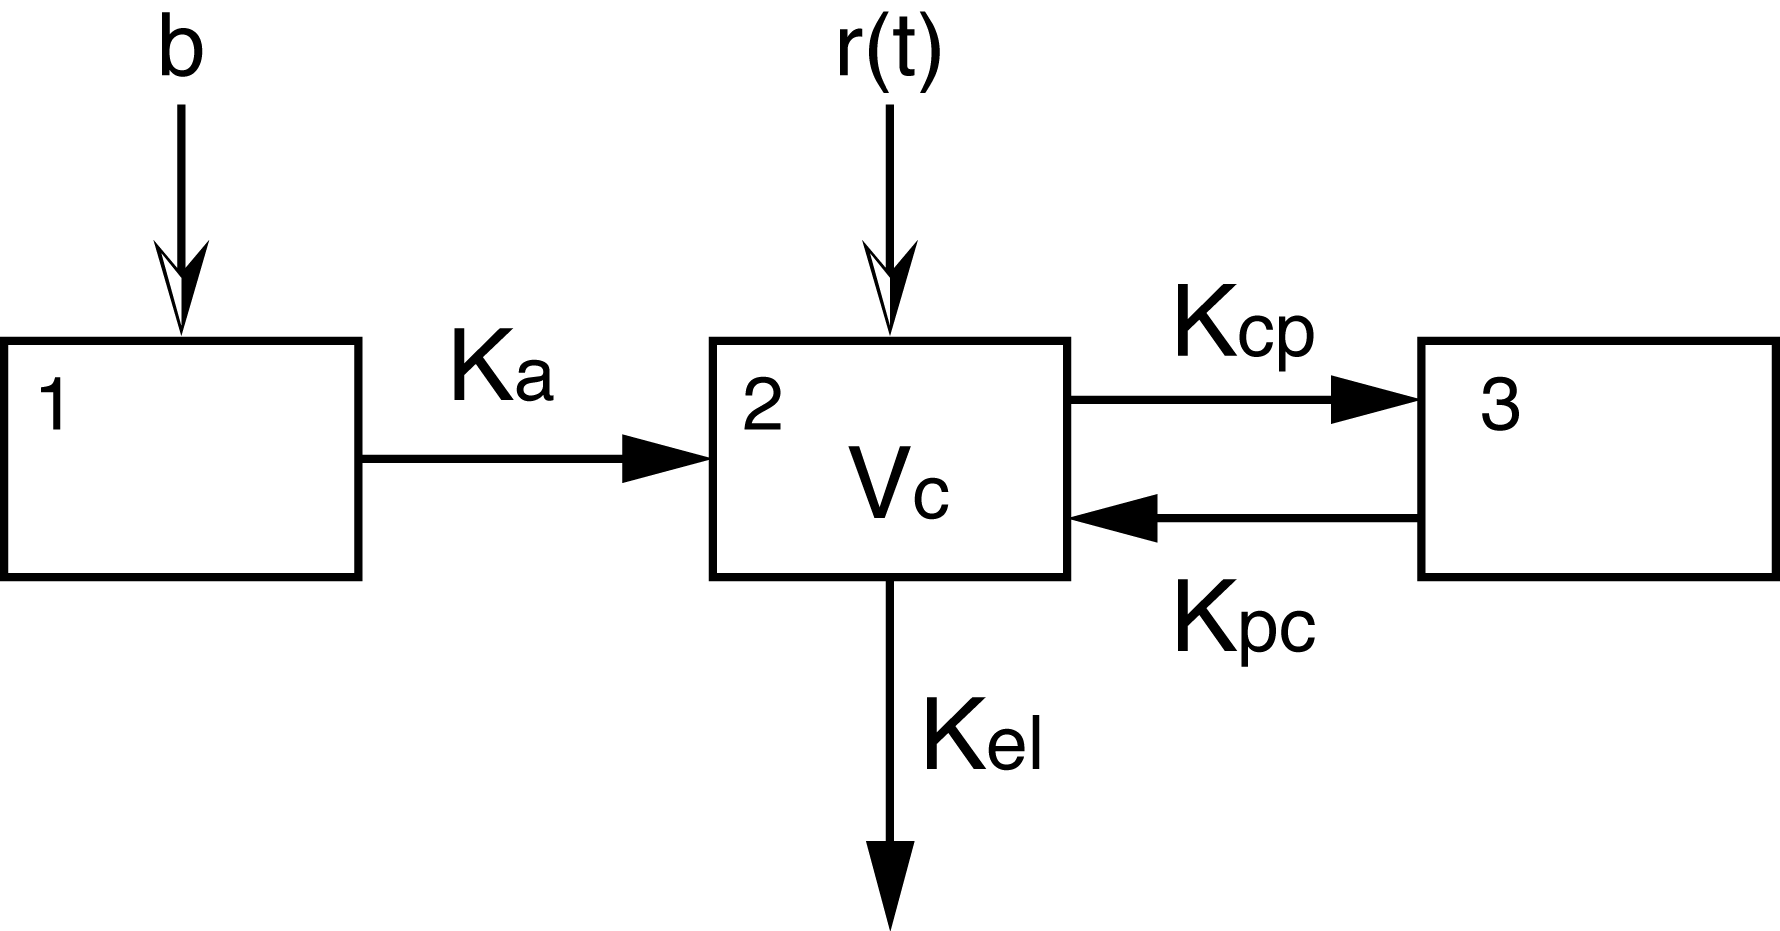
\includegraphics[scale=0.45, bb=0 0 1282 670]{figModel.png}
\caption{Model.
}
\label{Fig:Model}
\end{figure}


%
% Figure 002 -- Simulated output + Estimated vs. Simulated output
%
\begin{figure}[ht] % ebb generated bb=0 0 403 302
     \centering
        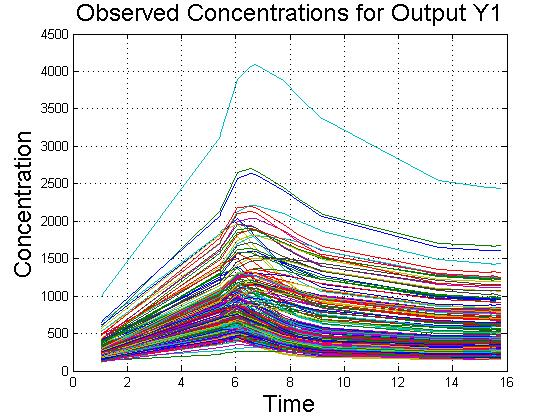
\includegraphics[width=0.65\linewidth, bb =0 0 603 452]{figRunBigObservedConcentrations.jpg}
        \caption{True simulated model profiles.}
        \label{Fig:Spaghetti}
\end{figure}

%
% Figure 003 -- Simulated Histograms
%
\begin{figure}[ht]
\centering
\begin{tabular}{@{}cc@{}} % ebb generated bb=0 0 403 302
\subfigure[$K_{el}$]{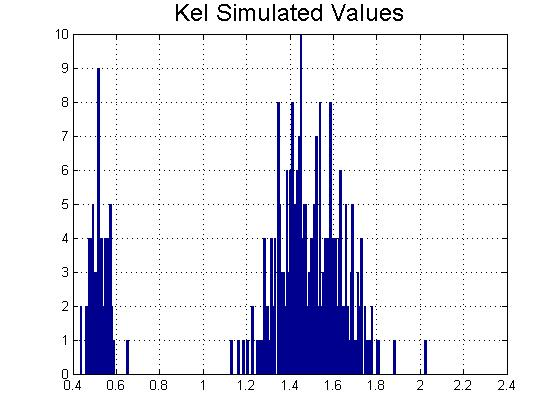
\includegraphics[width=0.3\textwidth, bb=-20 0 443 402]{figRunBigSimKEL.jpg}}     
\label{Fig:EstimatedKEL} & 
\subfigure[$V_{c}$]{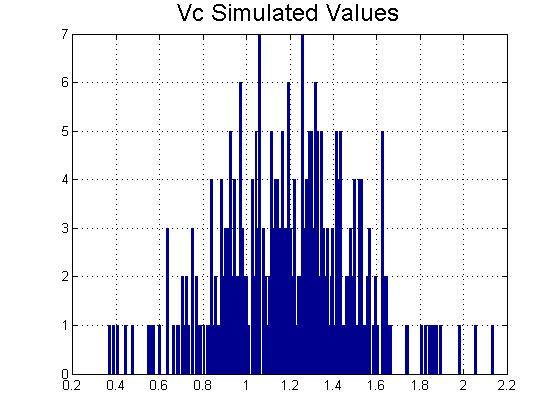
\includegraphics[width=0.3\textwidth, bb=-20 0 443 402]{figRunBigSimVOL.jpg}} 
\label{Fig:EstimatedVOL}\\
\subfigure[$K_{cp}$]{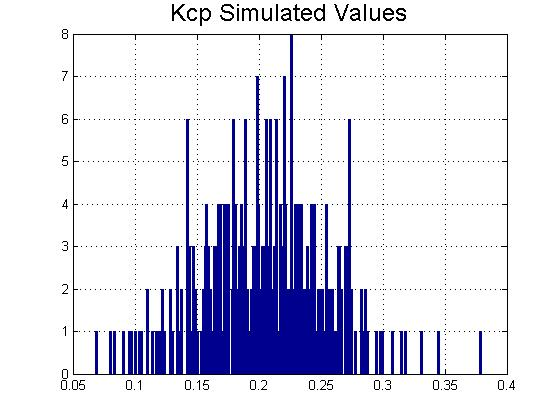
\includegraphics[width=0.3\textwidth, bb=-10 0 443 402]{figRunBigSimKCP.jpg}} 
\label{Fig:EstimatedKCP} &
\subfigure[$K_{pc}$]{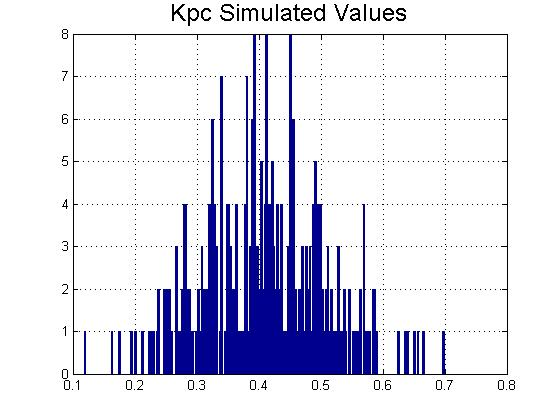
\includegraphics[width=0.3\textwidth, bb=-20 0 443 402]{figRunBigSimKPC.jpg}}
\label{Fig:EstimatedKPC} \\
\subfigure[$K_{a}$]{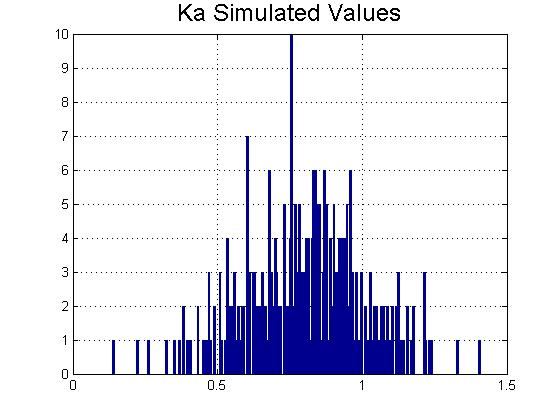
\includegraphics[width=0.3\textwidth, bb=-10 0 443 402]{figRunBigSimKA.jpg}}
\label{Fig:EstimatedPeripheralRateRatio}
\end{tabular}
\caption[]{Histogram of simulated PK parameters.}
\label{Fig:EstimatedPK}
\end{figure}

%
% Figure 004 -- Estimated Histograms
%
\begin{figure}[ht]
\centering
\begin{tabular}{@{}cc@{}} % ebb generated bb=0 0 864 648
\subfigure[$K_{el}$]{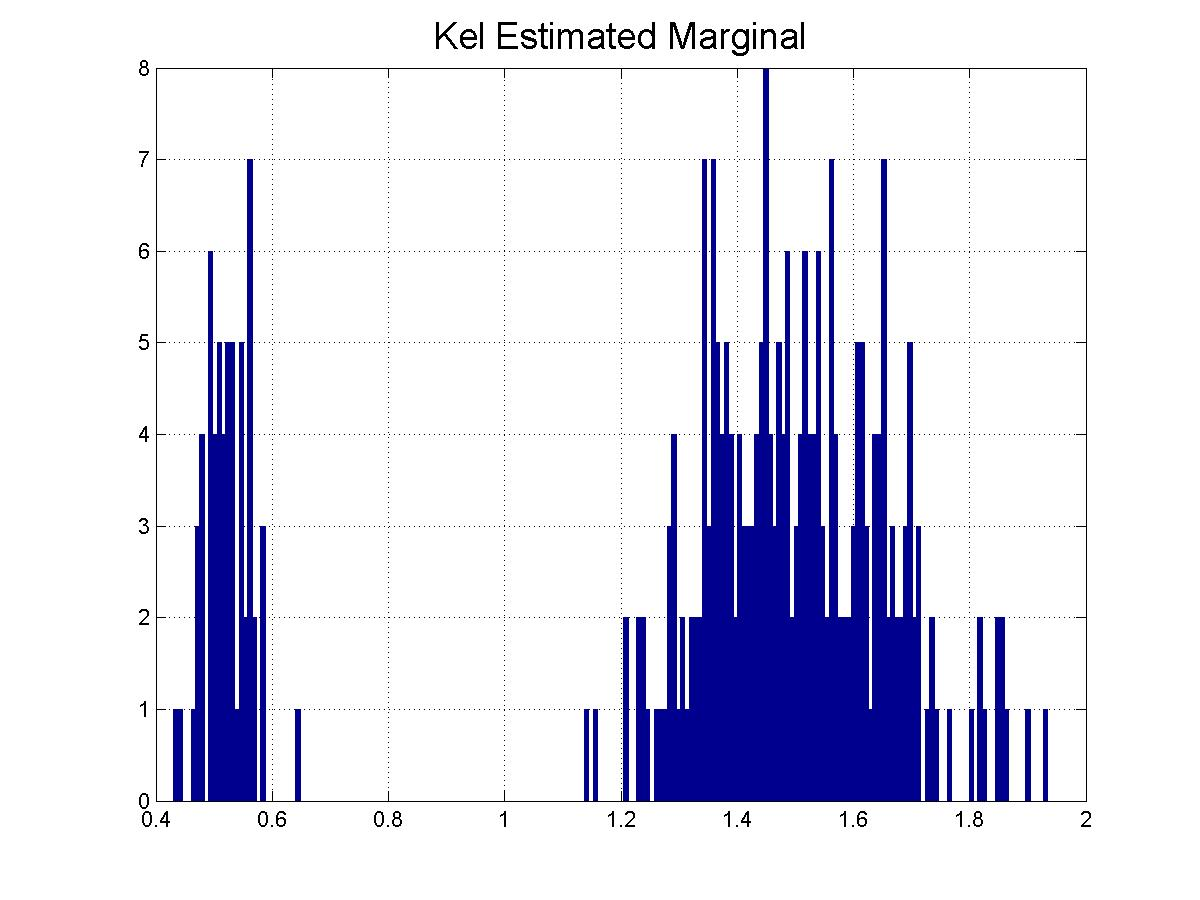
\includegraphics[width=0.3\textwidth, bb=-10 0 964 948]{figRunBigKEL_Est.jpg}}     
\label{Fig:SimulatedKEL} & 
\subfigure[$V_{c}$]{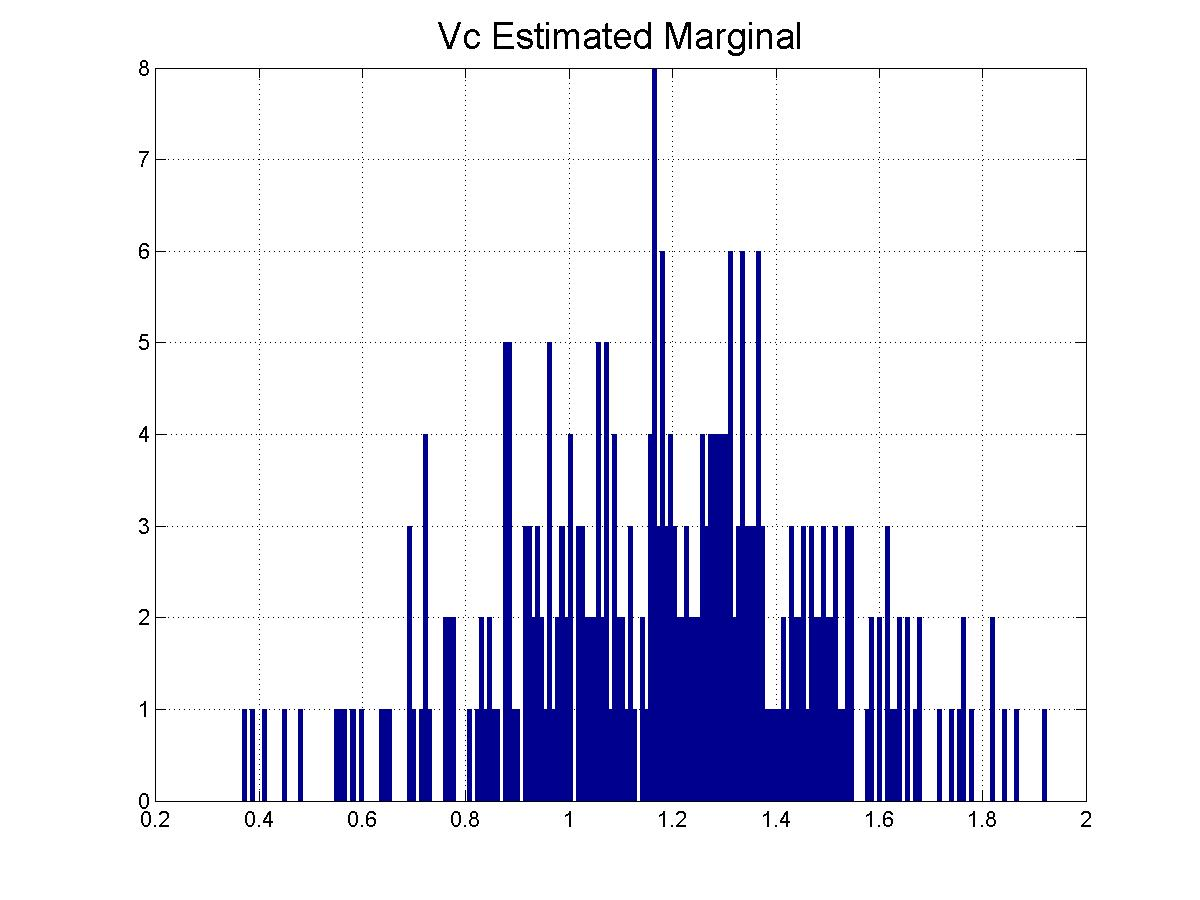
\includegraphics[width=0.3\textwidth,  bb=-10 0 964 948]{figRunBigVOL_Est.jpg}} 
\label{Fig:SimulatedVOL}\\
\subfigure[$K_{cp}$]{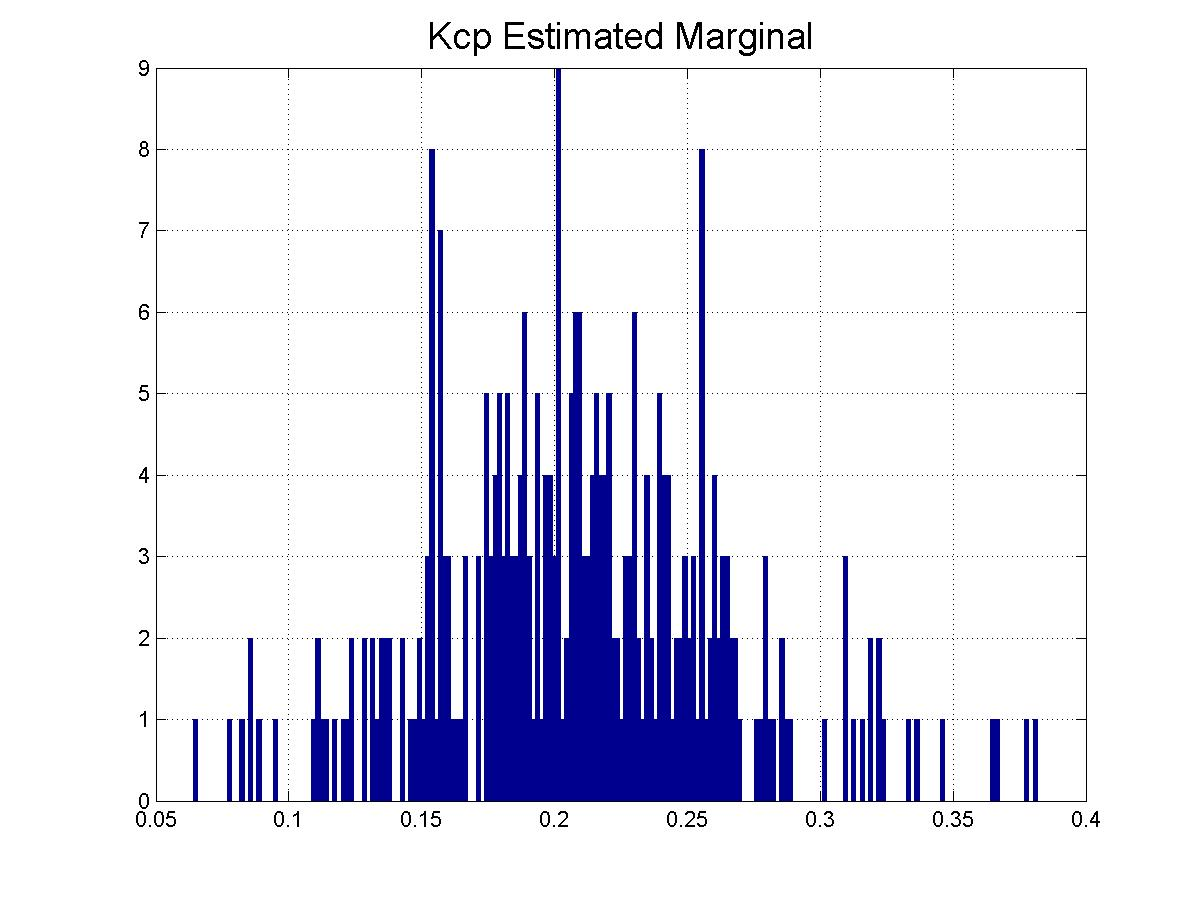
\includegraphics[width=0.3\textwidth,  bb=-10 0 964 948]{figRunBigKCP_Est.jpg}} 
\label{Fig:SimulatedKCP} &
\subfigure[$K_{pc}$]{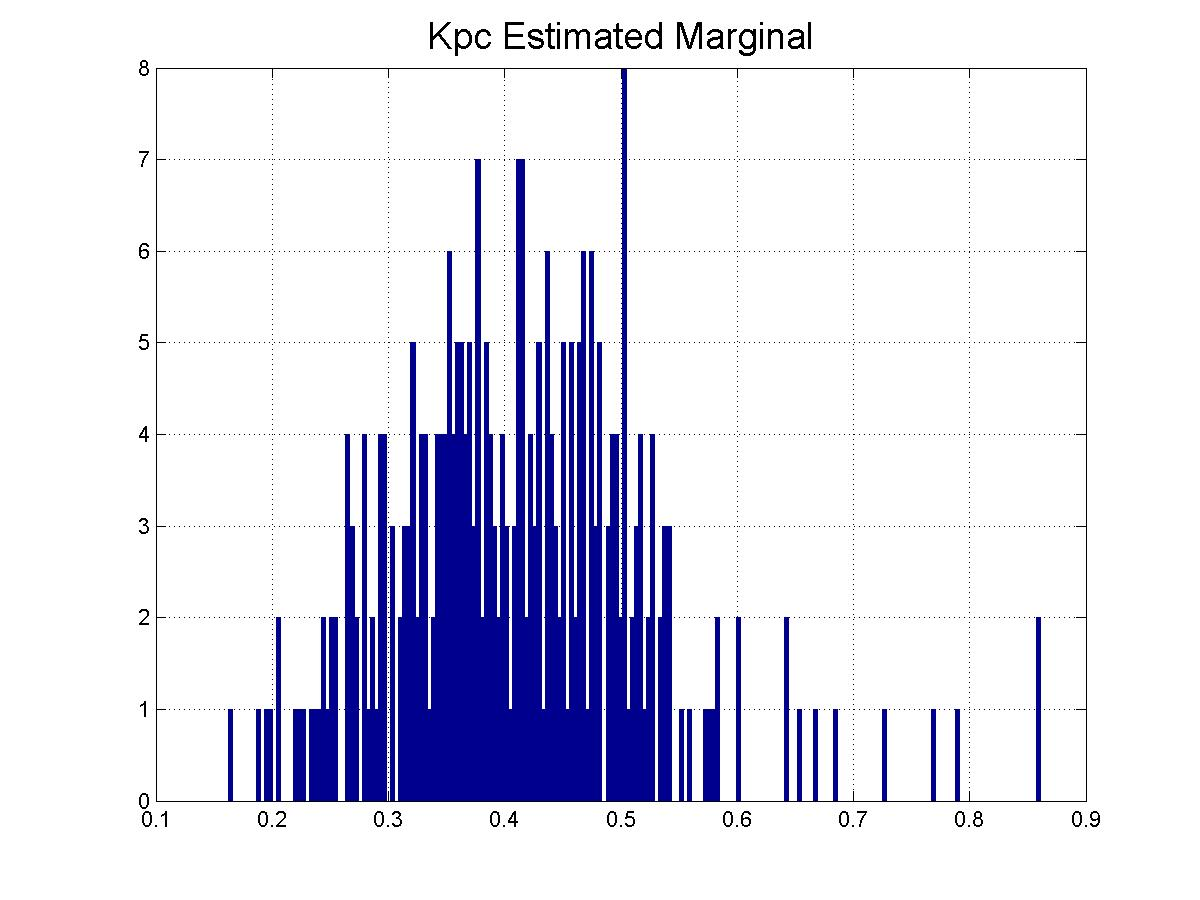
\includegraphics[width=0.3\textwidth,  bb=-10 0 964 948]{figRunBigKPC_Est.jpg}}
\label{Fig:SimulatedKPC} \\
\subfigure[$K_{a}$]{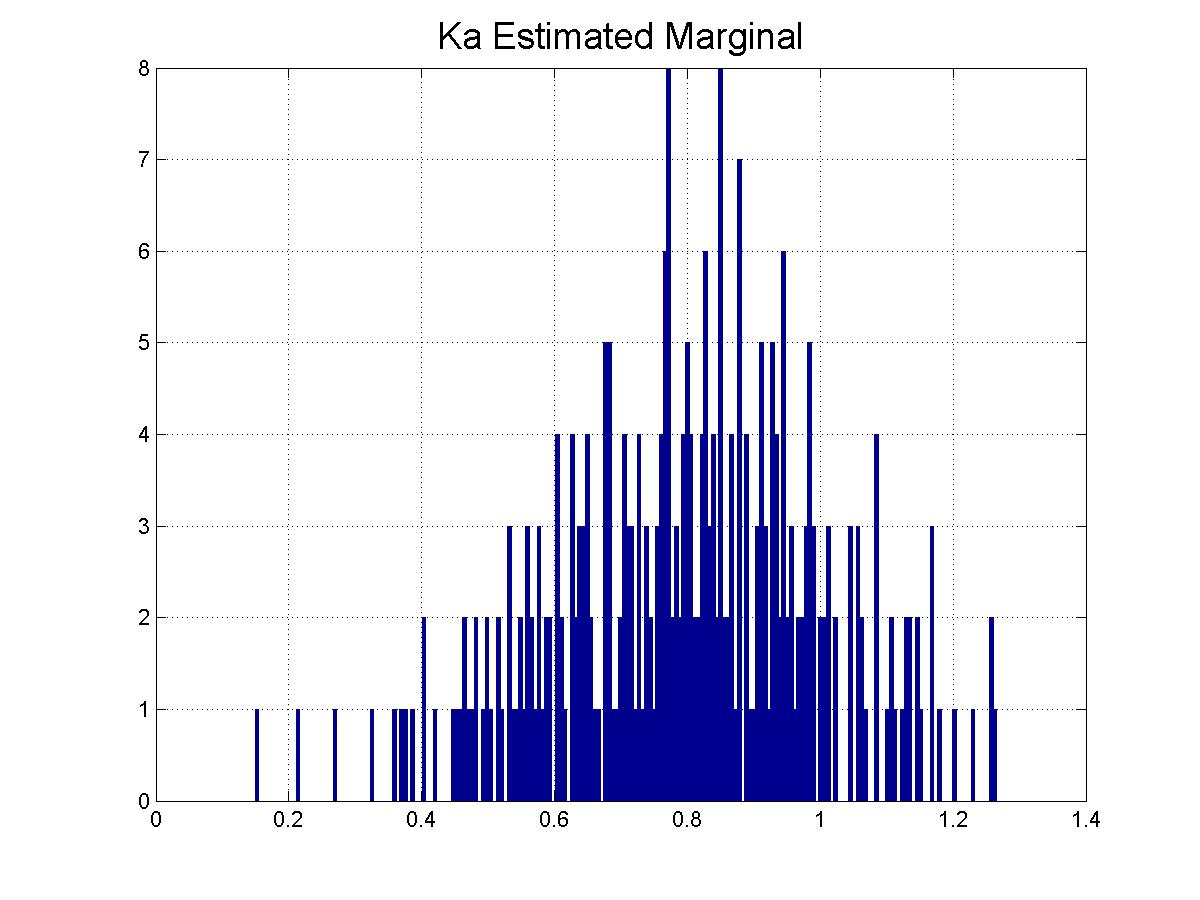
\includegraphics[width=0.3\textwidth,  bb=-10 0 964 948]{figRunBigKA_Est.jpg}}
\label{Fig:SimulatedPeripheralRateRatio} 
\end{tabular}
\caption[]{Estimated Marginals of PK parameters.}
\label{Fig:SimulatedPK}
\end{figure}

%
%  Figure 005 --  OP plot
%
\begin{figure}[ht] % original ebb bb=0 0 864 648
    \centering
        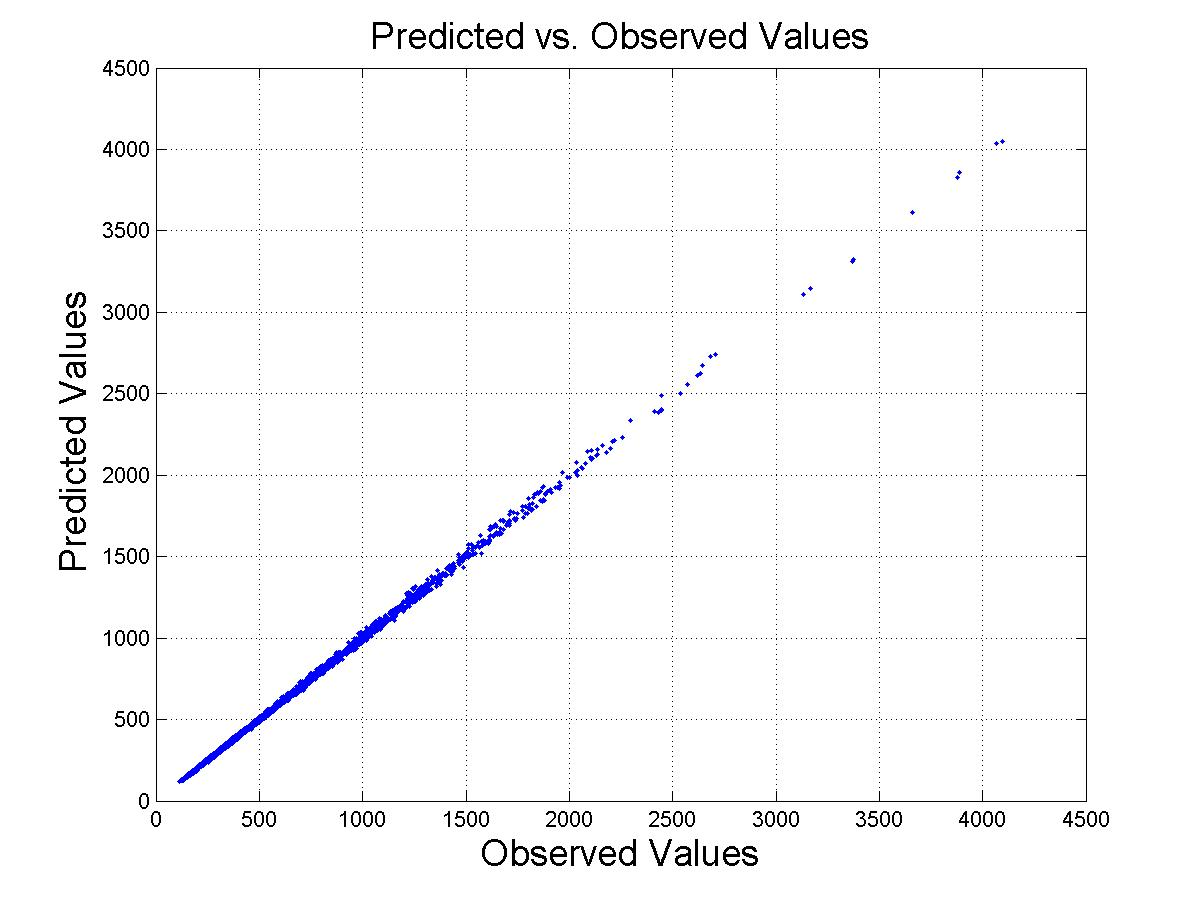
\includegraphics[width=0.65\linewidth, bb=0 0 1164 948]{figRunBigPredictedvsObserved3.jpg}
      \caption{Predicted vs. Observed.}
      \label{Fig:EstimatedvsSimulated}
\end{figure}

 \afterpage{\clearpage}

%%%%%%%%%%%%%%%%%%%%%%%%%%%%%%%%%%%%%%%%%%%%%%%%%%%

 \end{document}
